\documentclass[declaration,shortabstract,inz]{iithesis}

\polishtitle{Badanie gier kooperacyjnych z niepełną\fmlinebreak informacją na przykładzie gry ``Hanabi''}
\englishtitle{A study on cooperative games with incomplete\fmlinebreak information based on the game of ``Hanabi''}


\polishabstract {Od początku ery komputerów, gry planszowe były używane do~testowania limitów sztucznej inteligencji. W~ostatnich latach nadzwyczajną popularność, zarówno w~środowiskach pasjonatów gier planszowych, jak i~badaczy akademickich, zyskało Hanabi -~w~pełni kooperacyjna gra karciana z~niepełną informacją, którą można określić mianem ``kooperacyjnego pasjansa''. W~poniższej pracy przedstawiamy różnorodne metody tworzenia agentów grających w~Hanabi, którzy, przy surowych ograniczeniach na~czas wykonania ruchu, byliby zdolni do~gry na~poziomie ludzkiego gracza. W~tym celu zaimplementowaliśmy siedmiu agentów regułowych o~różnych stopniach zaawansowania wdrażanych strategii oraz agenta, który potrafi nauczyć~się gry bez ingerencji człowieka. Sprawdziliśmy także, w~jaki sposób strategie agentów wzajemnie na~siebie oddziałują. Badania empiryczne wykazały, że~stworzeni agenci potrafią grać na~poziomie zbliżonym do~ludzkiego, bez konieczności poświęcania wysokich nakładów mocy obliczeniowej. Pokazaliśmy również skuteczność metod uczących, które pozwoliły korzystającemu z~nich agentowi na~samoistne wypracowanie efektywnej strategii, osiągającej wyniki zbliżone do~tych uzyskiwanych przez ludzi. Aby ułatwić dalszą analizę zagadnienia, a~także umożliwić grę ze~stworzonymi agentami, wykonaliśmy graficzny interfejs użytkownika. Praca daje podstawy do~rozwijania problematyki wysokopoziomowej gry w~Hanabi z~ograniczeniami czasowymi i~stanowi funkcjonalny prototyp.}
%\englishabstract{\ldots}


\author{Wojciech Jarząbek\and Jacek Leja}
\advisor{dr Paweł Rychlikowski}
\date{\today}
% Data zlozenia pracy

\usepackage[utf8]{inputenc}
\usepackage{graphicx}
\usepackage{caption}
\usepackage{float}
\usepackage{array}
\usepackage{amsfonts}
\usepackage{spverbatim}

\graphicspath{{img/}}
\let\cleardoublepage=\clearpage

\begin{document}

\chapter{Wprowadzenie}

\section{Czym jest Hanabi?}

Gry planszowe to forma rozrywki, która towarzyszy człowiekowi od~tysięcy lat. Były one popularne już za~czasów starożytnych, czego dowodzi chociażby malowidło z~3300~r.~p.n.e, pochodzące z~grobowca Merknery, na~którym ukazano rozgrywkę Seneta. Przykładem może być także Królewska~Gra~z~Ur, której egzemplarze odnaleziono w~trakcie badań nad~starożytną Mezopotamią. Choć gry te zostały w~dzisiejszych czasach w~znacznej mierze zapomniane, nie~sposób nie~wspomnieć o~innych, które również istniały w~starożytności, takich~jak~warcaby czy~Go, a~także o~nieco młodszych szachach, które wciąż cieszą~się ogromną i~niesłabnącą popularnością.

Każdą z~tych gier łączy aspekt rywalizacji: pod~koniec rozgrywki jednoznacznie wyszczególnia~się jednego lub~więcej graczy, których określamy mianem zwycięzców, natomiast reszta -~przegrywa. Inny schemat prezentują gry kooperacyjne, gdzie zadaniem nie~jest pokonanie innych uczestników zabawy, a~osiągnięcie wspólnego celu, który gwarantuje wygraną. Można powiedzieć, że~przeciwnikiem graczy jest w~tym przypadku sama gra, która swoją konstrukcją skłania do~współpracy. Pierwsze gry tego typu powstały dopiero w~drugiej połowie XX~wieku i~początkowo miały wyłącznie charakter edukacyjny. Wraz z~popularyzacją tzw. ``planszówek'', gry kooperacyjne w~znacznym stopniu zyskały na~popularności, a~ich forma wyewoluowała w~kierunku rozrywki kładącej nacisk na~aspekty towarzyskie, które ograniczają lub~wręcz odrzucają współzawodnictwo. Przykładami takich gier mogą~być Pandemic, Martwa Zima, a~także Hanabi.

Hanabi (jap. fajerwerki) to~w~pełni kooperacyjna gra planszowa, która w~2013 roku wygrała prestiżową nagrodę Spiel~des~Jahres. Gracze wcielają~się w~niej w~pracowników fabryki fajerwerków, w~której omyłkowo zostały pomieszane ze~sobą różne rodzaje prochu. Celem jest złożenie w~odpowiedniej kolejności możliwie jak~największej ilości sztucznych ogni, które gracze otrzymują poprzez dobieranie kart z~potasowanej talii. Uczestnicy rozgrywki widzą karty, które są~w~posiadaniu innych graczy, lecz~nie~mogą przypatrywać~się~tym, którymi sami dysponują. Dodatkowo, komunikacja odnosząca~się do~treści kart podlega restrykcyjnym zasadom i~jest w~znacznym stopniu ograniczona, co~czyni rozgrywkę nietrywialną. Jakie strategie należy zatem zastosować, by~wygrać? Jak można przełożyć je~na~świat algorytmów?

\section{Hanabi a sztuczna inteligencja}

W~teorii gier istnieje pojęcie perfekcyjnego zagrania, czyli pojedynczego ruchu zależnego od~aktualnego etapu gry, prowadzącego do~stanu rozgrywki maksymalizującego oczekiwany wynik -~niezależnie od~ruchów, które mogą w~odpowiedzi wykonać inni gracze. Perfekcyjne zagrania są~podstawą optymalnego planu działania, minimalizującego możliwe straty ponoszone w~trakcie rozgrywania danej partii. Niestety, tak~silna strategia -~w~przypadku złożonych gier -~jest nieprawdopodobnie trudna do~uzyskania ze~względu na~ogromną rozpiętość drzewa możliwych do~uzyskania stanów rozgrywki. W~praktyce używa~się algorytmów: heurystycznych, regułowych, opartych na~technikach uczących, nadużywających zasad gry lub~siłowych. Przykładowo, słynny komputer Deep Blue, który w~maju 1997 roku pokonał ówczesnego mistrza świata w~szachach, Garrego Kasparova, nie~posiadał optymalnej strategii. Używał on~metody siłowej, wspomaganej algorytmem przeszukującym alfa-beta, rozpatrując wszystkie możliwe zagrania i~wybierając~te, które dawały mu~największą przewagę lokalną. Takie działanie było możliwe z~racji na~ogromną moc superkomputera, który potrafił rozpatrywać 200~milionów ruchów na~sekundę\cite{DeepBlue}.

Stworzenie agentów sztucznej inteligencji do~Hanabi to~zadanie, które wymaga pokonania trudności niespotykanych w~innych grach, takich jak: niepełnej informacji, losowości dobieranych kart, a~także ograniczonych zasobów, m.in. w~postaci podpowiedzi dla~innych graczy. Agenci muszą współpracować, gdyż gracz, który odmawia~kooperacji, może w~kilku ruchach doprowadzić do~przegranej całej grupy. Ważne jest, by~nie~marnować zasobów, a~zatem sztuczna inteligencja musi być odpowiednio skoordynowana. Ponadto, znikoma ilość kart w~talii nie~pozwala na~zbyt długą rozgrywkę -~oznacza to~zatem, że~aby zdążyć z~wygraną agenci muszą posiadać protokół komunikacji, który dopuszcza przekazywanie w~obrębie zasad gry dodatkowych, implicytnych informacji, rozumianych przez pozostałych jej~uczestników.

Niniejsza praca ma~na~celu zbadanie Hanabi jako gry kooperacyjnej z~niepełną informacją. Będziemy analizować techniki tworzenia agentów sztucznej inteligencji grających w~Hanabi, którzy wykonują możliwie najbardziej efektywne i~zrozumiałe dla ludzi ruchy na~tyle szybko, by~umożliwić komfortową rozgrywkę z~człowiekiem na~komputerach osobistych.


\chapter{Reguły gry}

\begin{figure}[ht!]
	\centering
	\captionsetup{format=hang}
	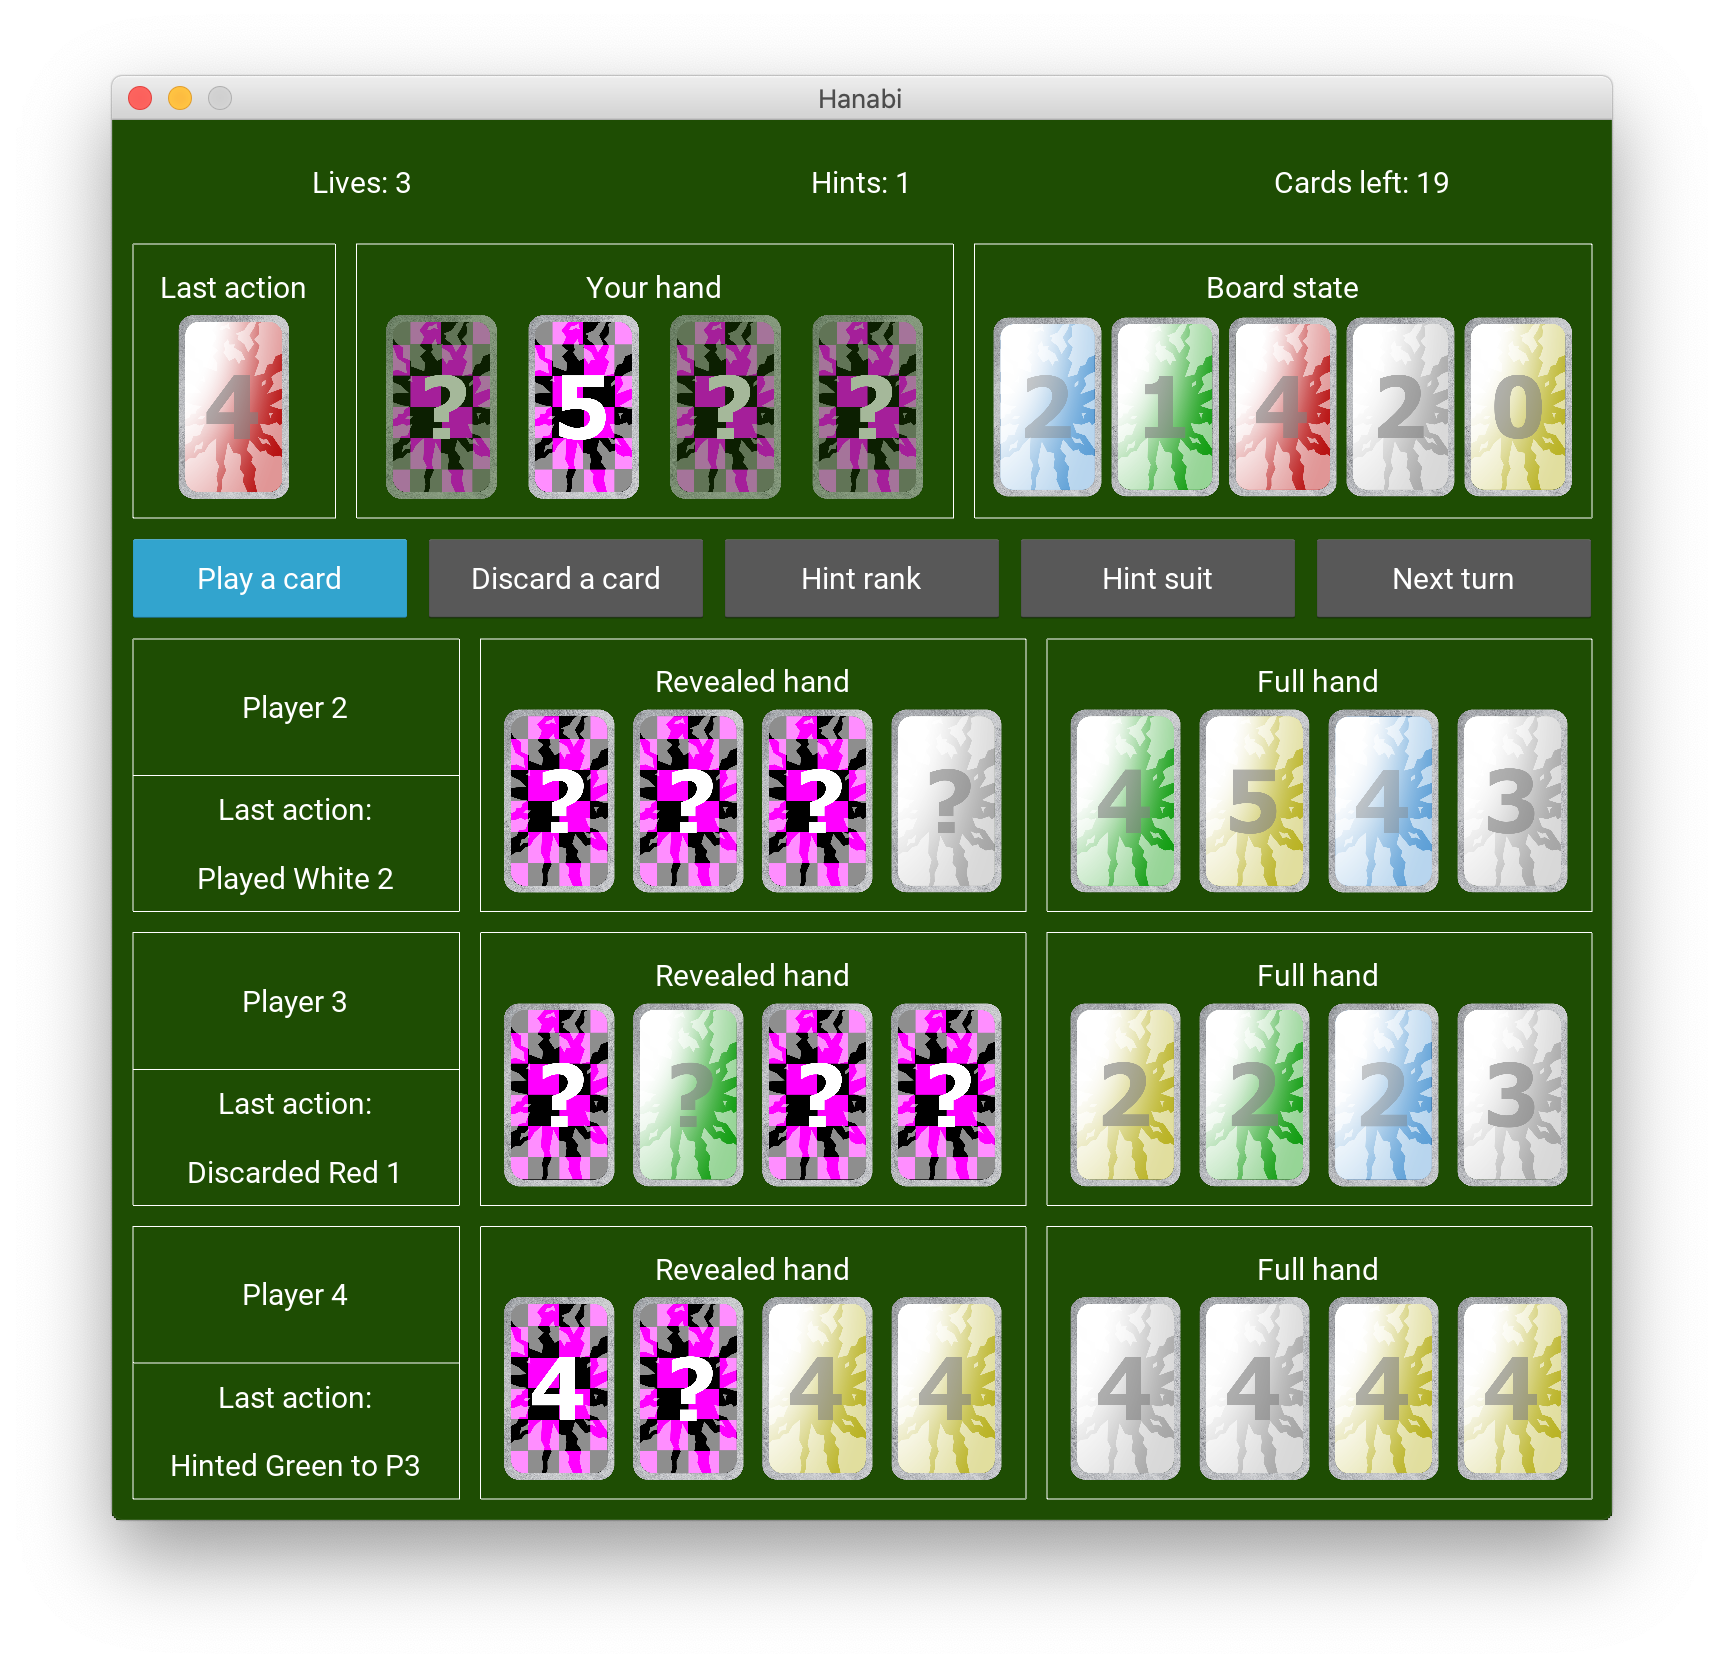
\includegraphics[width=\textwidth,height=\textheight,keepaspectratio]{gui.png}
	\caption[Caption]{Interfejs graficzny do gry Hanabi, utworzony na potrzeby projektu (twórca grafik: Jakub Podwysocki)}
	\label{fig:gui}
\end{figure}

\section{Wyjaśnienie zasad}

Celem gry jest zdobycie możliwie największej ilości punktów poprzez poprawne zagrywanie kart. Maksymalna ilość możliwych do~uzyskania punktów wynosi dwadzieścia pięć. Po~zakończeniu gry ilość uzyskanych punktów oblicza~się poprzez zsumowanie wartości najwyższych kart z~każdego ze~stosów odpowiedniego koloru.

Talia do~gry składa~się z~pięćdziesięciu kart. Każda karta jest~oznaczona jednym z~pięciu kolorów (czerwony, żółty, niebieski, biały, zielony) oraz jedną z~wartości z~zakresu od~1~do~5. Dla każdego koloru istnieją po~trzy karty o~numerze~1, po~dwie karty o~numerach 2,~3~i~4, a~także po~jednej karcie o~numerze~5.

Na początku gry talia jest tasowana. Gracze rozpoczynają rozgrywkę z~ośmioma żetonami podpowiedzi i~trzema żetonami życia. Żetony te~są~wspólne dla wszystkich uczestników rozgrywki. Jeżeli graczy jest dwóch lub~trzech, każdy z~nich dobiera po~pięć zakrytych kart. Jeżeli jest ich~czterech lub~pięciu, dobierają po~cztery zakryte karty. Następnie gracze po kolei wykonują swoje ruchy. Ruchu nie~można pominąć. Ruch to~wykonanie jednej z~trzech następujących akcji:
\begin{enumerate}
	\item Zagranie karty:

	Gracz deklaruje chęć wykonania zagrania, wybiera zakrytą kartę ze~swojej ręki, a~następnie wykłada ją~na~planszę w~pozycji odkrytej. Zagranie może być~poprawne lub~niepoprawne. Karty muszą być~zagrywane w~kolejności rosnącej, zaczynając od~jedynki, inaczej zagranie uważa~się za~niepoprawne. Przykładowo, jeśli na~planszy~nie ma~żadnych kart, można poprawnie zagrać tylko te, które są~oznaczone numerem~1. Jeżeli na~planszy znajdują~się wyłącznie jedna niebieska karta o~numerze~1 i~stos żółtych kart, spośród których największą wartość ma~karta o~numerze~4, można poprawnie zagrać niebieską kartę o~numerze~2, żółtą kartę o~numerze~5 lub dowolną kartę innego koloru o~numerze~1. Jeżeli karta została zagrana poprawnie, jest ona dodawana do~stosu o~odpowiednim kolorze lub~też~rozpoczyna stos swojego koloru, jeżeli jest to~karta o~numerze~1. Dodatkowo, jeżeli zagrana karta ma~numer~5, gracze otrzymują jeden żeton podpowiedzi (chyba, że~mają ich już osiem -~wtedy zagranie nie~ma~żadnego dodatkowego efektu). Jeżeli karta została zagrana niepoprawnie, jest ona~usuwana z~gry i~nie~jest dodawana do~żadnego ze~stosów, a~gracze tracą jeden z~żetonów życia. Po~rozpatrzeniu efektów zagrania gracz dobiera zakrytą kartę z~talii (jeżeli nie~jest ona~pusta).
	
	\item Odrzucenie karty:
 
	Gracz deklaruje chęć odrzucenia karty, wybiera zakrytą kartę ze~swojej ręki, a~następnie wykłada ją~na~planszę w~pozycji odkrytej. Karta ta~jest usuwana z~gry, bez dokładania jej~do~któregokolwiek ze~stosów, a~gracze otrzymują jeden żeton podpowiedzi (chyba, że~mają ich już osiem -~wtedy odrzucenie karty nie~ma~żadnego dodatkowego efektu). Po~rozpatrzeniu efektów akcji gracz dobiera zakrytą kartę z~talii (jeżeli nie~jest ona~pusta).

	\item Udzielenie podpowiedzi innemu graczowi:

	Gracz usuwa jeden z~żetonów podpowiedzi, następnie wybiera innego uczestnika rozgrywki oraz jeden z~dwóch rodzajów informacji, której chce mu~udzielić: może wskazać wszystkie jego karty o~wybranym kolorze lub~wszystkie jego karty o~wybranym numerze. Akcji tej nie~można wykonać, jeśli w~grze~nie ma~żadnych żetonów podpowiedzi, gdyż wiązałoby~się to~z~koniecznością usunięcia żetonu podpowiedzi, który~nie istnieje. Udzielanie graczom podpowiedzi dotyczących kart w~jakikolwiek inny sposób jest zabronione.
\end{enumerate}

Jeżeli któryś z graczy dobierze ostatnią kartę z~talii, każdy uczestnik rozgrywa jedną dodatkową turę (wraz z~graczem, który dobrał ostatnią kartę), a~następnie gra~się kończy.

Gra natychmiast kończy~się, gdy~zostanie utracony ostatni żeton życia lub gdy~wszystkie stosy odpowiednich kolorów zostaną skompletowane (czyli na~każdy z~nich poprawnie położono kartę o~numerze~5).

\section{Dodatkowe obserwacje}

Partie na~dwóch graczy cechują~się bardzo wysokim stopniem trudności. Uczestnicy rozgrywki znacznie częściej muszą radzić sobie ze~skomplikowanymi sytuacjami, które wynikają z~niekorzystnych rozdań. Fakt ten jest spotęgowany przez znikomą ilość dostępnych informacji (każdy z~graczy widzi naraz tylko pięć kart swojego sojusznika), a~także łatwość wpadnięcia w~cykl, w~którym jeden z~graczy udziela podpowiedzi, a~drugi zagrywa lub odrzuca karty.

Z~powodu losowej natury gry, w~niektórych rozdaniach nie~jest możliwe zdobycie maksymalnej ilością punktów. Najprostsza taka sytuacja ma~miejsce, gdy w~rozgrywce na~dwóch graczy jeden z~nich dobierze same karty o~numerze~5, drugi dobierze wyłącznie karty o~numerze~4, a~na~górze talii znajdują~się pozostałe karty o~numerze~4. Aby uzyskać dostęp do~kart o~innych numerach, gracze muszą odrzucić (lub niepoprawnie zagrać) co~najmniej sześć kart. Z~zasady szufladkowej Dirchleta można wywnioskować, że~wszystkie kopie co~najmniej jednej z~kart danego rodzaju zostaną bezpowrotnie usunięte z~gry, bez umieszczania ich na~stosie, co~uniemożliwi wygraną.

Ze~względu na~ograniczony rozmiar talii, zagrywanie wyłącznie tych kart, o~których posiada~się komplet informacji, jest wysoce nieefektywne. Po~rozdaniu kart talia zawiera od~30~do~40 kart, zależnie od~liczby graczy. Aby uzyskać najwyższy wynik, należy zagrać aż~25~kart, a~zagranie każdej z~nich oznacza zmniejszenie rozmiaru talii o~jeden. Oznacza to (zakładając, że~gracze próbują uzyskać 25~punktów), że~można wykonać maksymalnie od~10~do~17 ruchów, w~których odrzuca~się kartę, wliczając tury po~opróżnieniu talii. Po~doliczeniu początkowych 8~żetonów maksymalna ilość możliwych do~uzyskania podpowiedzi wynosi~25. Z~tego wynika, że~w~grze na~dwie osoby każda podpowiedź musi jednoznacznie ujawniać średnio po~jednej karcie, lecz każda z~nich potrzebuje dwóch podpowiedzi różnego rodzaju, by~uzyskać pełną informację. Przy pięciu graczach każda podpowiedź musi średnio ujawniać już nie~jedną, a~prawie półtorej karty.

Ponadto, jeżeli chcemy odrzucać wyłącznie karty, które można bezpiecznie usunąć z~gry, inni gracze muszą nam zakomunikować ich brak przydatności poprzez odpowiednie podpowiedzi (lub ich brak, co~jest w znacznym stopniu utrudnione przez konieczność udzielania pełnej informacji o~zawartości rąk współuczestników). Karty bezużyteczne mogą, lecz nie~muszą zostać ujawnione w~drodze przypadku, podczas ujawniania innych kart. W~rezultacie, najczęściej przyjmowaną konwencją wśród graczy jest odrzucanie najstarszej karty w~ręce: jeżeli żaden z~uczestników rozgrywki nie~ostrzega przed usunięciem jej z~gry, istnieje wysokie prawdopodobieństwo, że~jest ona nieprzydatna.

\chapter{Strategie sztucznej inteligencji}

\section{Podejście regułowe}

Podczas realnej rozgrywki Hanabi gracze nie~dysponują komputerem, który pomagałby im~w~wykonywaniu ruchów poprzez dokonywanie odpowiednich obliczeń. Zamiast tego korzystają oni z~wiedzy nabytej w~trakcie rozegranych już partii, modyfikując swoje strategie i~rozszerzając je~o~kolejne elementy, aż~do~osiągnięcia zadowalającego ich poziomu wiedzy o~grze. Proces ten w~naturalny sposób prowadzi do~wykształcenia konwencji (takich jak: ``należy zawsze odrzucać najstarszą kartę w~ręce''), a~także do~opracowania systemu reguł, pomocnych w~uzyskiwaniu wysokich wyników (przykładowo: ``jeżeli ktoś chce odrzucić ważną kartę, należy go~powstrzymać poprzez udzielenie odpowiedniej podpowiedzi''). Zasady te~można przełożyć na~algorytmy, co~prowadzi do~utworzenia systemów regułowych, znanych także jako eksperckie.

Algorytmy regułowe to~programy, naśladujące poprzez procesy decyzyjne wybory, których w~danych sytuacjach mógłby dokonać człowiek. Są~one najczęściej deterministyczne, co~jest cechą szczególnie ważną w~środowiskach, które wymagają koordynacji i~przewidywania działań podejmowanych przez inne elementy systemu. W~przypadku agentów sztucznej inteligencji, algorytmy regułowe powielają zachowania prawdziwych graczy.

Z~racji na kooperacyjną konstrukcję Hanabi, sama emulacja typowych zachowań ludzkich graczy~nie wystarcza, by~wygrać. Potrzebna jest także odpowiednia koordynacja działań pomiędzy agentami: strategia. Gracze muszą zwracać uwagę na~współuczestników rozgrywki i~na~bieżąco interpretować ich poczynania, by~móc wywnioskować, jaka seria ruchów doprowadzi do~najlepszej możliwej sytuacji. Prostym i~efektywnym sposobem na~zaimplementowanie strategii jest wyszczególnienie protokołu komunikacji pomiędzy agentami, który nadaje niektórym zagraniom dodatkowe znaczenie, rozumiane przez pozostałych graczy. Przykładowo, skuteczna może być zasada o~następującej treści: ``jeżeli inny gracz podpowiedział mi~bez wyraźnej przyczyny jeden z~kolorów, ujawniając w~ten sposób kilka kart, najprawdopodobniej mogę je~zagrać, w~kolejności od~lewej do~prawej''. Z~tego powodu implementacja agentów regułowych wiąże~się z~koniecznością bardzo dobrej znajomości zasad rządzących grą.

\section{Drzewa poszukiwań}

Istnieją dwa główne czynniki, które sprawiają, że~analiza stanu gry w~Hanabi jest trudnym zadaniem. Są~to: niepełna informacja o~aktualnym etapie rozgrywki, a~także losowość kart dobieranych z~talii. Udowodniono, że~nawet w~uproszczonej wersji gry, w~której uczestnicy mogą patrzeć na~swoje karty, problem perfekcyjnego zagrania jest NP-kompletny\cite{NP-Complete}. Sprawia to, że~próba rozwiązania zagadnienia w~sposób siłowy jest nieefektywna. Fakt ten, połączony z~trudnością opracowania funkcji oceniającej jakość zagrania, wyklucza użycie części możliwych rozwiązań problemu, takich jak algorytm alfa-beta.

Aby zredukować trudność znalezienia perfekcyjnego zagrania, grupa Facebook Research zaproponowała rozwiązanie bazujące na~drzewie poszukiwań Monte Carlo\cite{MCTS}. Każdy z~graczy dysponuje zbiorem predefiniowanych akcji, dostosowywanych odpowiednio do~aktualnego stanu rozgrywki poprzez analizę prawdopodobieństwa zagrań, które mogą wykonać współuczestnicy. Algorytm bierze pod uwagę także szanse aktualnego gracza na~posiadanie w~ręce kart, które mogły zostać wylosowane z~talii. Aby przyspieszyć działanie programu, głębokość drzewa poszukiwań jest ograniczana, a agenci wykonują predefiniowane akcje i~nie~eksplorują nowych opcji, jeśli wiązałoby~się to~z~przekroczeniem zadanego limitu obliczeń.

Takie podejście pozwala na~uzyskanie bardzo wysokich wyników, sięgających nawet 24.61~punktów w~rozgrywce dla dwóch graczy. Działanie algorytmu jest jednak kosztowne obliczeniowo, nawet przy znacznym ograniczeniu zakresu dokonywanych poszukiwań. Do~osiągnięcia tak wysokich punktacji potrzeba olbrzymich ilości obliczeń, które, z~racji na możliwość ich zrównoleglenia, są~najczęściej dokonywane na~nowoczesnych kartach graficznych. Wyłączenie agentom możliwości dokonywania dodatkowych poszukiwań degeneruje ich do~postaci agentów regułowych, którzy, choć na~każdą akcję potrzebują zużycia istotnie mniejszej ilości zasobów, wciąż osiągają imponujący wynik 23~punktów.

\section{Algorytmy uczące}

Innym sposobem na~zaimplementowanie programu grającego w~Hanabi jest użycie algorytmów uczących, które łączą zalety podejść regułowych i~poszukujących. Jak sugeruje nazwa, polegają one na~symulowaniu procesu akumulacji doświadczenia, podobnego do~tego doznawanego przez ludzkich graczy. W~toku ewolucji agent zdobywa wiedzę o~środowisku, w~którym operuje, dostosowując~się do~zmieniających warunków oraz wypracowując i~udoskonalając sposoby radzenia sobie w~zaprezentowanych sytuacjach. Tworzenie algorytmów uczących nie~wymaga ani szerokiej wiedzy o~zawiłościach zasad gry, ani kosztownych obliczeń, które byłyby wykonywane w~trakcie rozgrywki.

Wadą tego algorytmu jest konieczność wyuczenia agenta odpowiednich zachowań. Odbywa~się to~poprzez zapewnienie mu~zestawu danych, na~których mógłby zdobyć doświadczenie. W~zależności od~uzyskiwanych wyników, decyzje algorytmu są~nagradzane lub karane. Dobranie odpowiednio różnorodnego zbioru uczącego, w~parze z~funkcjami kwalifikującymi, pozwala programowi nie~tylko na~rozpoznawanie i~radzenie sobie z~najczęściej występującymi sytuacjami, ale i~generalizację zachowań, potrzebną do~wybrnięcia ze~stanów gry, które nie~zostały dotychczas napotkane.

Należy pamiętać, że~nieodpowiedni dobór zbioru uczącego lub funkcji, które oceniają poczynania agenta, potrafi doprowadzić do~anomalii w~procesie zdobywania wiedzy. Jeżeli zestawy testowe będą zbyt homogeniczne i~zbyt liczne w~stosunku do~osiągalnej liczby stanów rozgrywki, może dojść do~przeuczenia modelu, z~kolei zbyt krótka nauka nie~przygotuje programu do~nietypowych sytuacji. Nieprawidłowości w~procedurach klasyfikujących, choć mniej zauważalne, także potrafią doprowadzić do~niepożądanych sytuacji, tak jak miało to~miejsce w~przypadku programu grającego w~produkcje na~platformę Nintendo Entertainment System. Agent ten, nie~chcąc doprowadzić do~przegranej, nauczył~się wstrzymywać rozgrywkę na~zawsze\cite{Mario}.

\section{Naginanie zasad gry}

W~oficjalnych zasadach gry nie~ma~wyszczególnionego przymusu udzielania podpowiedzi, które ujawniałyby jakiekolwiek karty. Jeżeli wybierzemy gracza, który nie~posiada żadnych czerwonych kart i~zdecydujemy się na~podpowiedzenie mu~czerwonego koloru, tura jest pomijana za~cenę żetonu podpowiedzi. Choć taki ruch wydaje~się~nie mieć sensu, gdyż podpowiedź można wykorzystać w~produktywny sposób, otwiera on~możliwość poważnego nagięcia zasad gry. Jeżeli każdej z~możliwych podpowiedzi przypiszemy unikatową wartość numeryczną, możemy za~ich pomocą przekazywać innym graczom informacje liczbowe. Jest to~powód, dla~którego możliwość udzielania pustych podpowiedzi jest uznawana w~społeczności graczy Hanabi za~kontrowersyjną, toteż w~niektórych edycjach gry została ona zakazana.

Fakt ten można wykorzystać do~stworzenia agenta, który za~pomocą pozornie bezwartościowych ruchów udziela podpowiedzi wszystkim graczom jednocześnie. Korzysta on~ze~słynnej zagadki logicznej, znanej jako problem więźniów i~kapeluszy, odpowiednio uogólnionej i~dopasowanej do~liczby graczy. Agent, który rozgrywa aktualną turę, oblicza idealne zagrania dla~innych uczestników rozgrywki, a~następnie szyfruje je~do~postaci liczbowej. Kolejni gracze, znając podaną przez poprzednika wartość, po~rozpatrzeniu optymalnych zagrań innych graczy, są~w~stanie wywnioskować, jaki ruch powinni wykonać.

Według badań z 2017 roku\cite{HatPlayer}, agent ten uzyskuje maksymalną ilość punktów średnio w~92\%~rozgrywanych gier, co~jest wynikiem bliskim optymalnemu. To~imponujący rezultat, zarówno ze~względu na~bardzo szybkie działanie algorytmu, jak i~jego nadzwyczajną efektywność.

Niestety, taki sposób gry całkowicie zawodzi, gdy jeden z~graczy wyłamie~się z~konwencji narzuconej przez protokół komunikacji. Dodatkowo, algorytm działa wyłącznie w~rozgrywkach na~czterech oraz pięciu graczy, gdyż głównym powodem jego sukcesu jest możliwość przekazywania w~każdej z~podpowiedzi maksymalnej ilości informacji, toteż~zmniejszenie liczby graczy powoduje znaczne zredukowanie efektywności ruchów. Są~to~powody, dla których agent ten nie~nadaje~się do~rozgrywki z~człowiekiem.

\chapter{Funkcjonalna realizacja SI}

W~celu zbadania zaprezentowanych sposobów tworzenia sztucznej inteligencji, która potrafiłaby grać w~Hanabi, zaimplementowaliśmy dziewięciu agentów. Aby umożliwić testowanie ich możliwości, opracowaliśmy także graficzny interfejs (patrz: \hyperref[fig:gui]{Rysunek 2.1}), pozwalający użytkownikowi na~aktywne uczestnictwo w~rozgrywce, złożonej z~dowolnie dobranego przez niego składu graczy komputerowych.

Siedmiu agentów jest opartych o~systemy regułowe, różniące~się stopniem zaawansowania wdrażanych strategii. Aby usprawnić działanie jednego z~agentów regułowych, użyliśmy bayesowskiej metody optymalizacji hiperparametrów, korzystającej z~procesów gaussowskich. Ostatni z~zaprezentowanych agentów stosuje algorytm uczący ze~wzmocnieniem, oparty o~funkcje heurystyczne generalizujące stan gry, wspomagane procesami decyzyjnymi Monte Carlo.

Systemy zasad zostały oparte o~nasze własne spostrzeżenia, zdobyte poprzez obserwację rozgrywek ludzkich graczy, które uznaliśmy za~kluczowe do~gry na~wysokim poziomie. Każdy kolejny agent regułowy bazuje na~konceptach, które zostały użyte do~zbudowania jego poprzedników, i~usprawnia je. Takie działanie~prowadzi do~naturalnej progresji warstw abstrakcji prezentowanych pojęć.

\subsection*{Nomenklatura}

\begin{tabular}{@{}>{$}l<{$}@{ --- }l@{}}
	\mu & średnia arytmetyczna \\
	\tilde{\mu} & mediana \\
	\sigma^2 & wariancja \\
	\sigma & odchylenie standardowe \\
\end{tabular}

\newpage

\section{Cheater}

Cheater jest agentem, którego strategia polega na~bezmyślnym oszukiwaniu. Program oszukuje, dzięki czemu zawsze posiada komplet informacji o~kartach, którymi dysponuje, lecz~nie wykorzystuje dostępnej mu~wiedzy w~optymalny sposób: zagrywa karty, gdy to~możliwe, w~przeciwnym wypadku losowo je~odrzuca.

\subsection*{Nowe pojęcia}

\begin{itemize}

	\item \textbf{Legalna akcja}:
	
	Jeżeli wybrana akcja może być wykonana w~danym momencie rozgrywki, jest ona legalna, niezależnie od~poprawności. Przykładowo: udzielenie informacji w~momencie, w~którym na~planszy nie~znajduje~się ani jeden żeton podpowiedzi, jest nielegalne. Jeżeli akcja jest nielegalna, korespondująca z~nią część algorytmu kończy~się niepowodzeniem.
	
	\item \textbf{Ujawniona karta}:
	
	Jeżeli gracz dysponuje kartą, o~której posiada komplet informacji, kartę tę~określimy jako ujawnioną.
	
	\item \textbf{Bezpieczna akcja}:
	
	Jeżeli gracz może wykonać ruch, który nie doprowadzi do~utraty żetonów życia, taką akcję określimy jako bezpieczną.
	
	\item \textbf{Bezpieczne zagranie}:
	
	Jeżeli gracz posiada ujawnioną kartę, którą może bezpiecznie (czyli poprawnie) położyć na~planszy, wykonanie takiej akcji nazwiemy bezpiecznym zagraniem.
\end{itemize}

\subsection*{Schemat działania}

\begin{enumerate}
	\item Podejrzyj posiadane karty.
	\item Jeżeli posiadasz bezpieczne zagranie, wykonaj je.
	\item Odrzuć losową kartę.
\end{enumerate}

\subsection*{Osiągi}

\begin{figure}[H]
	\centering
	\captionsetup{format=hang}
	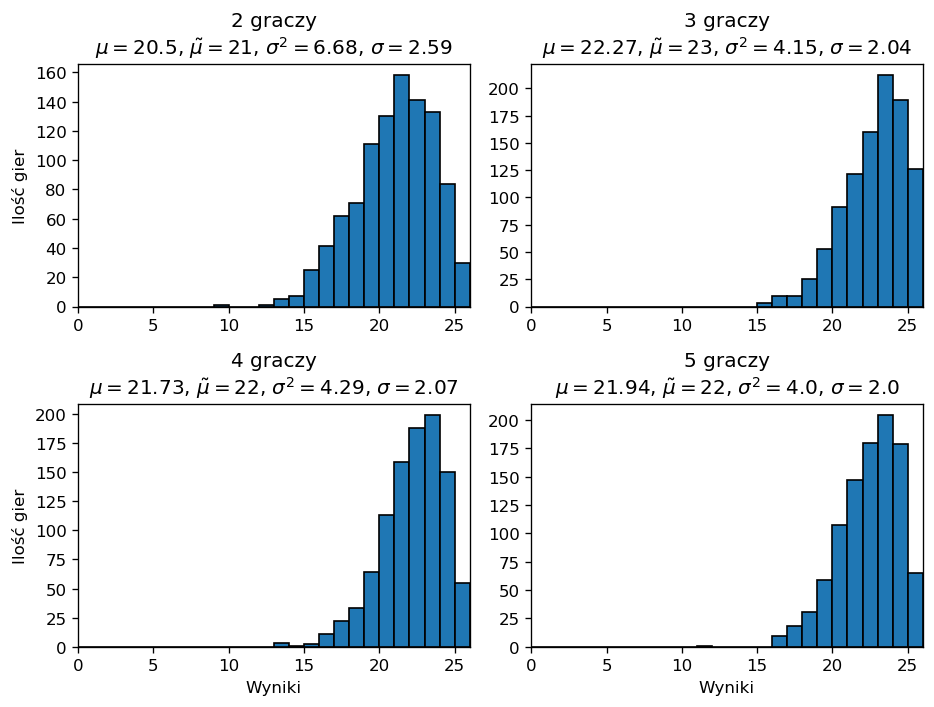
\includegraphics[width=\textwidth,height=\textheight,keepaspectratio]{Cheater.png}
	\caption[Caption]{Wyniki agenta Cheater (rozmiar próby: 1000 gier)}
	\label{fig:Cheater}
\end{figure}

Uzyskane wyniki są~bardzo dobre, lecz cechują~się stosunkowo wysoką wariancją. Agenci są~skłonni do~odrzucania kluczowych kart i~nie~zwracają uwagi na~fakt, że~może to~znacząco utrudnić lub nawet uniemożliwić dalsze zdobywanie punktów.

\section{SmartCheater}

SmartCheater usprawnia poczynania agenta Cheater. Program oszukuje, dzięki czemu zawsze posiada komplet informacji o~kartach, którymi dysponuje, i~wykorzystuje tę~wiedzę w~sposób bliski optymalnemu, stosując strategię przedłużającą rozgrywkę. Agent potrafi oceniać przydatność kart i~za~wszelką cenę unika ruchów, które utrudniają lub uniemożliwiają wygraną.

\subsection*{Nowe pojęcia}

\begin{itemize}
	\item \textbf{Zagranie lawinowe}:
	
	Jeżeli położenie karty na~planszy pozwala innym graczom na~wykonywanie nowych ruchów, które kontynuują dokładanie kart do~stosów, takie zagranie nazwiemy lawinowym. Przykładowo: jeżeli aktualny gracz poprawnie zagra czerwoną kartę o~numerze~1, a~dwaj kolejni gracze posiadają kolejno czerwone~karty o~numerach~2~i~3, zagranie jest lawinowe.
	
	\item \textbf{Bezużyteczna karta}:
	
	Jeżeli nie~istnieje i~nie będzie istniała możliwość poprawnego zagrania karty, jest ona bezużyteczna i~może być odrzucona bez żadnych konsekwencji. Przykładowo: gdy stos kart koloru zielonego jest w~pełni ułożony, nie~można poprawnie zagrać żadnych dodatkowych kart koloru zielonego.
	
	\item \textbf{Karta krytyczna}:
	
	Jeżeli karta nie~jest bezużyteczna i~nie istnieją już inne jej kopie, które można by~zagrać, karta jest krytyczna. Przykładowo: każda karta o~numerze~5 jest krytyczna.
	
	\item \textbf{Spasowanie tury}:
	
	Jeżeli na~planszy znajduje~się co~najmniej jeden żeton podpowiedzi, udzielenie losowej podpowiedzi dowolnemu z~graczy jest równoznaczne ze~spasowaniem tury, gdyż nie~jest dobierana żadna nowa karta (chyba, że~dobrano ostatnią kartę z~talii).
\end{itemize}

\subsection*{Schemat działania}

\begin{enumerate}
	\item Podejrzyj posiadane karty.
	\item Jeżeli posiadasz bezpieczne zagranie, wykonaj je. Pierwszeństwo nadawane jest zagraniom lawinowym, a~w~razie konfliktu wygrywa losowa karta o~najniższym numerze.
	\item Jeżeli możesz spasować turę, a~ruch ten~nie~przeszkodzi żadnemu z~pozostałych graczy w~wykonaniu jednej z~akcji od~2~do~5, zrób to.
	\item Jeżeli posiadasz bezużyteczną kartę, odrzuć ją.
	\item Jeżeli jest to~możliwe, spasuj turę.
	\item Jeżeli posiadasz kartę, której kopia znajduje się w~ręce innego gracza, odrzuć ją.
	\item Jeżeli posiadasz kartę, która nie~jest krytyczna, odrzuć ją.
	\item Odrzuć losową kartę krytyczną o~najwyższym numerze.
\end{enumerate}

\subsection*{Osiągi}

\begin{figure}[H]
	\centering
	\captionsetup{format=hang}
	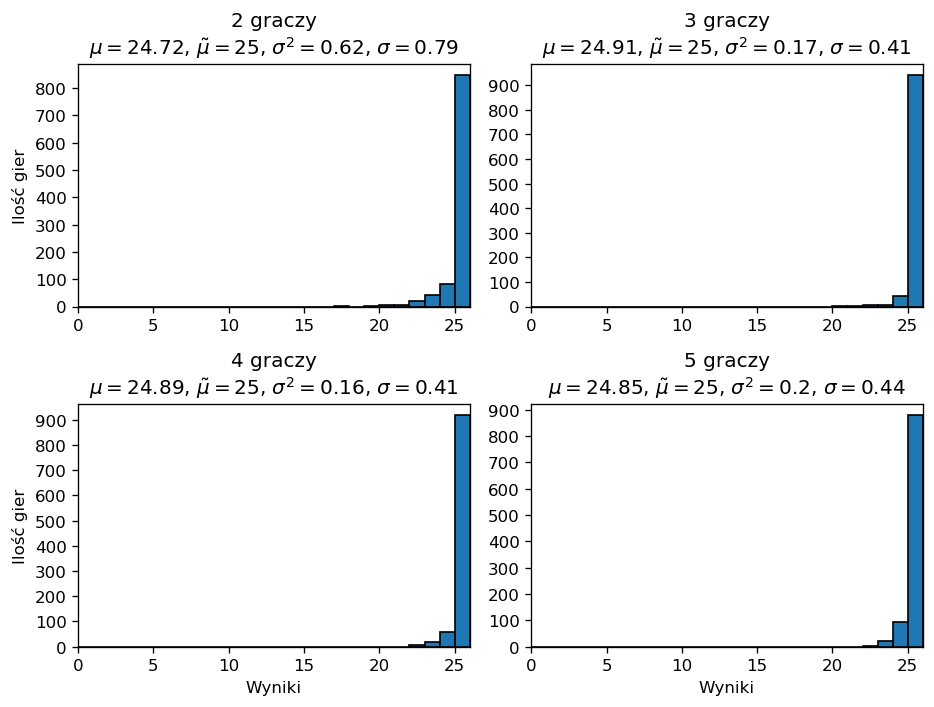
\includegraphics[width=\textwidth,height=\textheight,keepaspectratio]{SmartCheater.png}
	\caption[Caption]{Wyniki agenta SmartCheater (rozmiar próby: 1000 gier)}
	\label{fig:SmartCheater}
\end{figure}

Jak można oczekiwać po~agencie, który posuwa~się do~oszustwa bliskiego doskonałemu, jego wyniki są~bardzo wysokie -~nawet w~przypadku partii na~dwóch graczy, które cechują~się największymi dysproporcjami w~rozgrywce. Warto zauważyć, że~istnieją rozdania cechujące~się tak wysokim stopniem trudności, że~nawet ten agent uzyskuje w~nich mniej niż 20~punktów.

\section{Erratic}

Strategia agenta Erratic polega na~wykonywaniu serii przypadkowych ruchów, które są~legalne.

\subsection*{Schemat działania}

\begin{itemize}
	\item Wylosuj jedną z~legalnych akcji (zagraj kartę, odrzuć kartę, udziel podpowiedzi innemu uczestnikowi rozgrywki).
	\item Losowo wybierz szczegóły ruchu, a~następnie go~wykonaj.
\end{itemize}


\subsection*{Osiągi}

\begin{figure}[H]
	\centering
	\captionsetup{format=hang}
	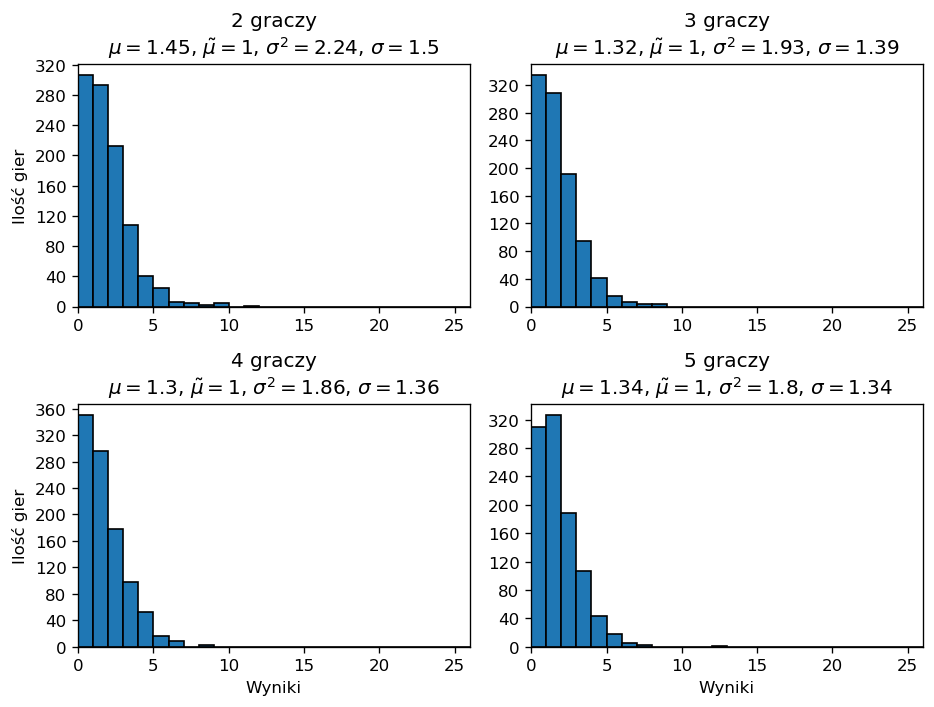
\includegraphics[width=\textwidth,height=\textheight,keepaspectratio]{Erratic.png}
	\caption[Caption]{Wyniki agenta Erratic (rozmiar próby: 1000 gier)}
	\label{fig:Erratic}
\end{figure}

Agent wykonujący wyłącznie losowe ruchy jest pierwszym tu~opisanym, który nie~oszukuje. Niestety, jak można było przewidywać, przegrywa on~większość gier, uzyskując wynik 0~punktów. Jest to~spowodowane brakiem mechanizmu, który powstrzymywałby go~przed zagrywaniem kart, które nie~są~bezpieczne, toteż zagrania mają małą szansę na~bycie poprawnymi. Choć istnieje szansa na~wykonanie akcji udzielenia podpowiedzi, które w~tym przypadku są~bezużyteczne, ruch nie~zaburza wyników, gdyż wykorzystanie żetonu podpowiedzi nie~prowadzi do~eskalacji progresu gry (jeżeli nie~dobrano ostatniej karty z~talii).

\section{StoppedClock}

Agent StoppedClock rozszerza strategię agenta Erratic: wykonuje losowe ruchy, które nie~mogą doprowadzić do~utraty żetonów życia. Jego postępowanie, choć nadal bardzo chaotyczne, czasem prowadzi do~wysokich punktacji, zgodnie z~maksymą: ``nawet zepsuty zegar dwa razy na~dobę pokazuje właściwą godzinę''.

\subsection*{Schemat działania}

Ruch agenta polega na~zbadaniu, które z~trzech dostępnych akcji są~legalne, a~następnie wylosowaniu i~wykonaniu jednej z~nich. Ponieważ tylko druga i~trzecia akcja mogą wzajemnie~się wykluczać, gracz zawsze będzie w~stanie wykonać co~najmniej jeden z~ruchów. Dostępne akcje to:

\begin{itemize}
	\item Jeżeli posiadasz bezpieczne zagranie, wykonaj je.
	\item Odrzuć losową kartę, priorytetyzując tę, która ma najmniej ujawnionych informacji. Akcja nie~może być wykonana, jeżeli na~planszy znajduje~się osiem żetonów podpowiedzi.
	\item Wybierz losowego gracza, który posiada co~najmniej jedną kartę o~niepełnej informacji, wylosuj jedną, po~czym losowo podpowiedz kolor lub numer wybranej karty, jeżeli nie~zostały one uprzednio ujawnione. Jeżeli wszyscy gracze posiadają komplet informacji, spasuj turę.
\end{itemize}

\subsection*{Osiągi}

\begin{figure}[H]
	\centering
	\captionsetup{format=hang}
	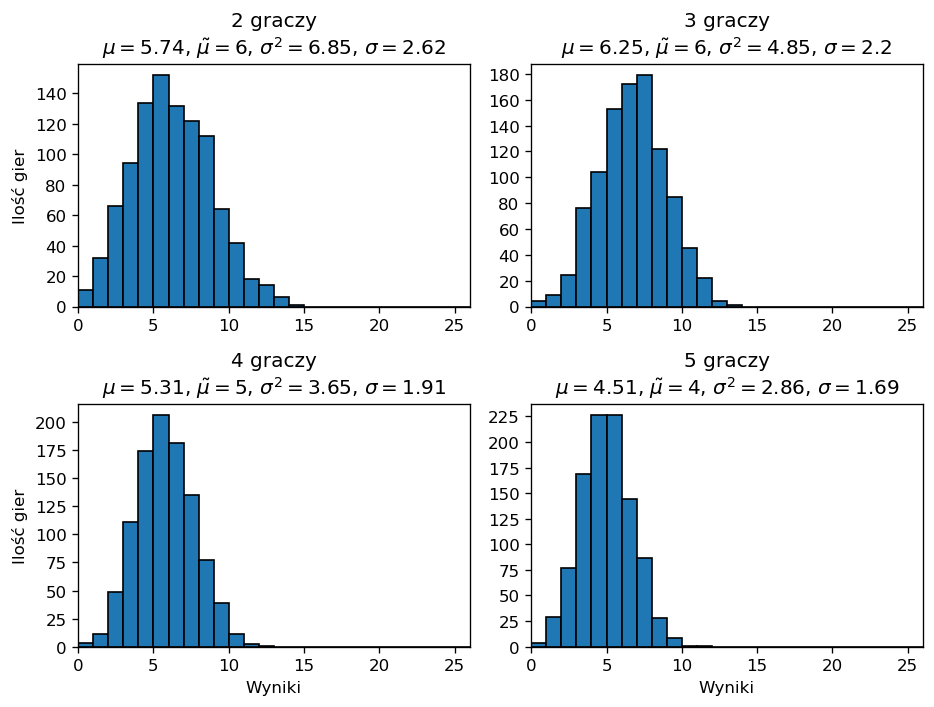
\includegraphics[width=\textwidth,height=\textheight,keepaspectratio]{StoppedClock.png}
	\caption[Caption]{Wyniki agenta StoppedClock (rozmiar próby: 1000 gier)}
	\label{fig:StoppedClock}
\end{figure}

Agent ma~nikłą szansę na~uzyskanie wysokich wyników, a~jego konstrukcja nigdy nie~pozwoli na~wygraną. Jest to~spowodowane ograniczeniem, które umożliwia programowi funkcjonowanie: wykonywane ruchy muszą być bezpieczne, co~koliduje z~ograniczoną liczbą żetonów podpowiedzi.

\section{SimpleDistrustful}

Agent SimpleDistrustful imituje postępowanie człowieka, który po~raz pierwszy gra w~Hanabi: wykonuje wyłącznie bezpieczne ruchy, lecz robi to~umiejętnie, gdyż potrafi przeprowadzać pewne wnioskowania, które na~jego miejscu mogłyby dokonać osoby o~podstawowej znajomości zasad. Program nie~udziela zbędnych podpowiedzi, stroni od~odrzucania kart, które mogą~się jeszcze przydać, a~także rozumie, że~niektóre karty zawsze można bezpiecznie zagrać lub odrzucić -~mimo posiadania o~nich niepełnej informacji.

\subsection*{Nowe pojęcia}

\begin{itemize}
	\item \textbf{Inferowalna karta}:

	Użyteczności niektórych kart można dociec poprzez analizę aktualnego stanu rozgrywki. Przykładowo: na~początku gry zawsze można zagrać dowolną kartę z~numerem~1, niezależnie od~tego, czy jej kolor został ujawniony. Podobnie, jeżeli nie~odrzucono ani nie zagrano żadnej karty o~numerze~4, żadna taka karta nie~może być krytyczna. Karty o~takiej właściwości nazywamy inferowalnymi, czyli dającymi~się wywnioskować. W~pełni ujawnione karty są~trywialnie inferowalne.
	
	\item \textbf{Wartościowa podpowiedź}:
	
	Zdarzają się~sytuacje, w~których udzielanie pewnych informacji jest niepożądane. Przykładowo: jeżeli dwóch lub więcej uczestników rozgrywki posiada kopię danej karty, warto skupić~się na~ujawnianiu wyłącznie jednej z~nich. Wartościowa podpowiedź to~taka, która jest lokalnie optymalna, gdyż unika powtarzania znanych informacji.
	
	\item \textbf{Najbliższy gracz}:
	
	Uczestnik rozgrywki, który po~zakończeniu akcji aktualnego gracza wykona ruch najwcześniej.
	
\end{itemize}

\subsection*{Schemat działania}

\begin{enumerate}
	\item Jeżeli posiadasz inferowalnie bezpieczne zagranie, wykonaj je.
	\item Jeżeli jest to~możliwe, wybierz najbliższego gracza, któremu możesz udzielić wartościowej podpowiedzi, a~następnie zrób to, nadając priorytet kartom o~niższych numerach.
	\item Jeżeli posiadasz nieujawnioną kartę, odrzuć ją.
	\item Jeżeli posiadasz kartę, która nie jest inferowalnie krytyczna, odrzuć ją.
	\item Odrzuć losową kartę.
\end{enumerate}

\subsection*{Osiągi}

\begin{figure}[H]
	\centering
	\captionsetup{format=hang}
	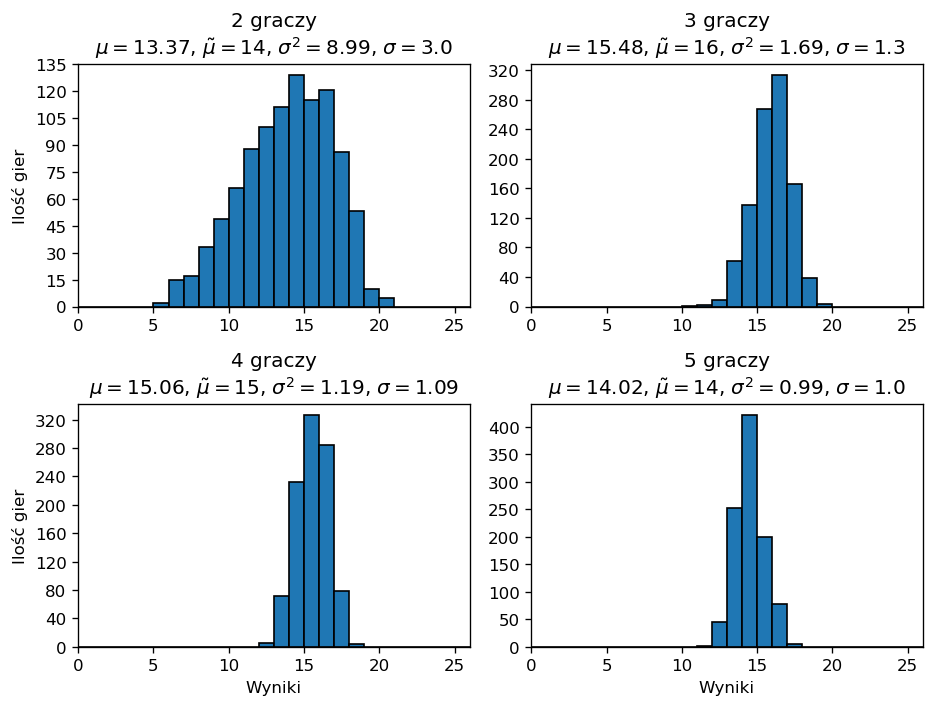
\includegraphics[width=\textwidth,height=\textheight,keepaspectratio]{SimpleDistrustful.png}
	\caption[Caption]{Wyniki agenta SimpleDistrustful (rozmiar próby: 1000 gier)}
	\label{fig:SimpleDistrustful}
\end{figure}

Agent nie~uzyskuje wysokich wyników, gdyż opiera swoje działania na~przeciętnej strategii. Udzielanie wyłącznie wartościowych informacji skłania graczy do~zagrywania kart, lecz często nie~wystarcza do~ochrony kart krytycznych -~nieujawnione karty wymagają pewnej formy ochrony, gdyż mogły być dobrane dopiero niedawno. Szczególnie zawodzą wyniki rozgrywek dla dwóch graczy, które cechują~się nadzwyczaj wysoką niestabilnością.

\section{Distrustful}

Agent Distrustful dopracowuje strategię stosowaną przez SimpleDistrustful. Program nadal gra zachowawczo, lecz ma~do~dyspozycji maksymalnie rozszerzony system dedukcji. Aby zminimalizować prawdopodobieństwo odrzucania kart krytycznych, został on~dodatkowo usprawniony o~konwencję, która chroni najnowsze karty poprzez nadawanie im~wysokich priorytetów. Aby zwiększyć potencjalną przydatność każdej z~dokonywanych akcji, agent dynamicznie dostosowuje swój sposób postępowania do~aktualnego stanu rozgrywki i~zmienia priorytety manewrów, w~zależności od~ilości pozostałych żetonów podpowiedzi. Pozwala to~na~dopasowywanie przyjmowanej taktyki, przy jednoczesnym zachowaniu zasad ugruntowanych przez narzuconą strategię.

\subsection*{Nowe pojęcia}

\begin{itemize}
	\item \textbf{Pułap jakościowy}:
	
	Jedna z~miar używanych w~funkcjach oceniających przydatność ruchów: jeżeli uzyskana przez daną akcję nota jest niższa od~pułapu, to~jest ona dyskwalifikowana jako niewystarczająco pomocna. 

	\item \textbf{Heurystycznie wartościowa akcja}:
	
	Niektóre akcje, takie jak bezpieczne zagranie, w~oczywisty sposób mają korzystny wpływ na~uzyskanie wyższego wyniku gry. Niestety, przypisanie części ruchów jednoznacznej wartości liczbowej, wskazującej na jej przydatność w~kontekście danego momentu rozgrywki, jest trudnym zadaniem, gdyż pełna analiza możliwych następstw akcji wymagałaby wysokiego nakładu mocy obliczeniowej. Aby uniknąć tego problemu, można zastosować funkcje heurystyczne, które przybliżają wartości poszukiwanych~ocen. Akcja, która uzyska najwyższą notę, a~także będzie wyższa od~zadanego pułapu jakościowego, jest nazywana heurystycznie wartościową.
	
	\item \textbf{Najstarsza (najmłodsza) karta}:
	
	Karta, która znajduje~się w~ręce danego gracza od~największej (najmniejszej) ilości tur, w~porównaniu do~innych jego kart. W~razie konfliktu za~najstarszą (najmłodszą) kartę uznawana jest ta~wysunięta najbardziej na~lewo (prawo).

\end{itemize}

\subsection*{Schemat działania}

Agent jest złożony z~siedmiu modułów, które są~rozważane po~kolei w~jednej z~trzech konfiguracji. Każdy moduł, poza ostatnim w~sekwencji, może zawieść. Ich kolejność zależy od~ilości posiadanych żetonów podpowiedzi:

\begin{itemize}
	\item Mniej niż 3~żetony: sekwencja 1, 2, 5, 3, 4, 7 (moduł 6 nie jest używany).
	\item Od~3~do~7 żetonów: sekwencja 1, 2, 3, 4, 5, 6, 7.
	\item Dokładnie 8~żetonów: sekwencja 1, 2, 3, 4, 6, 5, 7.
\end{itemize}

\newpage

\noindent Używane moduły to:

\begin{enumerate}
	\item \underline{``Necessary tip''}:
	
	Jeżeli najbliższy gracz planuje w~kolejnym ruchu odrzucić kartę krytyczną, która mogłaby zostać poprawnie zagrana, powstrzymaj go~poprzez udzielenie odpowiedniej podpowiedzi.

	\item \underline{``Obvious play''}:
	
	Jeżeli posiadasz inferowalnie bezpieczne zagranie, wykonaj~je, nadając priorytet kartom o~niższych numerach.

	\item \underline{``Good play tip''}:
	
	Jeżeli posiadasz co~najmniej dwa żetony podpowiedzi i~istnieje heurystycznie wartościowa podpowiedź, udziel jej, nadając priorytet tym, które umożliwią inferowalnie bezpieczne zagranie.

	\item \underline{``Discard tip''}:
	
	Jeżeli posiadasz co~najmniej dwa żetony podpowiedzi i~istnieje heurystycznie wartościowa podpowiedź, która umożliwi innemu graczowi odrzucenie inferowalnie bezużytecznej karty, udziel jej.

	\item \underline{``Obvious discard''}:
	
	Jeżeli posiadasz inferowalnie bezużyteczną kartę, odrzuć ją.

	\item \underline{``Mediocre play tip''}:
	
	Jeżeli posiadasz co~najmniej dwa żetony podpowiedzi, wykonaj akcję modułu numer~3 (``Good play tip''), ale ze~znacznie niższym pułapem jakościowym.

	\item \underline{``Guess discard''}:
	\begin{enumerate}
		\item Jeżeli posiadasz nieujawnione karty, odrzuć najstarszą z~nich.
		\item Jeżeli posiadasz karty, które nie~są~inferowalnie krytyczne, odrzuć najstarszą z~nich.
		\item Odrzuć najstarszą kartę.
	\end{enumerate}

\end{enumerate}

Zmiana kolejności manewrów pozwala na~kontrolowanie priorytetów agenta: im~mniej żetonów podpowiedzi znajduje~się w~grze, tym bardziej nagląca staje~się potrzeba ich odzyskania. Nigdy~nie wiadomo, czy i~kiedy któryś z~graczy dobierze kartę wymagającą natychmiastowej interwencji w~formie dodatkowych informacji. Jest to~powód, dla którego moduły, udzielające podpowiedzi do~kart niebędących krytycznymi, zawodzą przy próbie wykorzystania ostatniego z~żetonów.

Każda z~kart jest oceniana z~osobna przy użyciu funkcji heurystycznych. Za~ostateczną wartość podpowiedzi przyjmuje~się sumę ocen wszystkich kart, które zostaną za~jej pomocą ujawnione. Wagi funkcji heurystycznych zostały dobrane eksperymentalnie. Na~werdykt algorytmu wpływają między innymi następujące czynniki:
\begin{itemize}
	\item stopień ujawnienia karty,
	\item numer karty,
	\item czy zagranie karty jest lawinowe,
	\item czy podpowiedź jest wartościowa,
	\item ilość kart, które muszą być zagrane, zanim zagranie karty będzie bezpieczne,
	\item odległość właściciela karty od~gracza udzielającego podpowiedzi.
\end{itemize}

Początkowo, moduł numer~1 (``Necessary tip'') przyjmował inną formę. Agent był szczególnie ostrożny i~zawsze ostrzegał kolejnego gracza, jeżeli ten mógł odrzucić kartę krytyczną. W~praktyce doprowadzało to~do~powstawania cykli, w~których gracze naprzemiennie udzielali podpowiedzi i~odrzucali karty, przez co~częstotliwość zagrań drastycznie spadała. Choć pierwotny moduł znacznie pogarszał wyniki agenta Distrustful, jego zrewidowana wersja jest punktem centralnym kolejnego, bardziej zaawansowanego agenta.

\subsection*{Osiągi}

\begin{figure}[H]
	\centering
	\captionsetup{format=hang}
	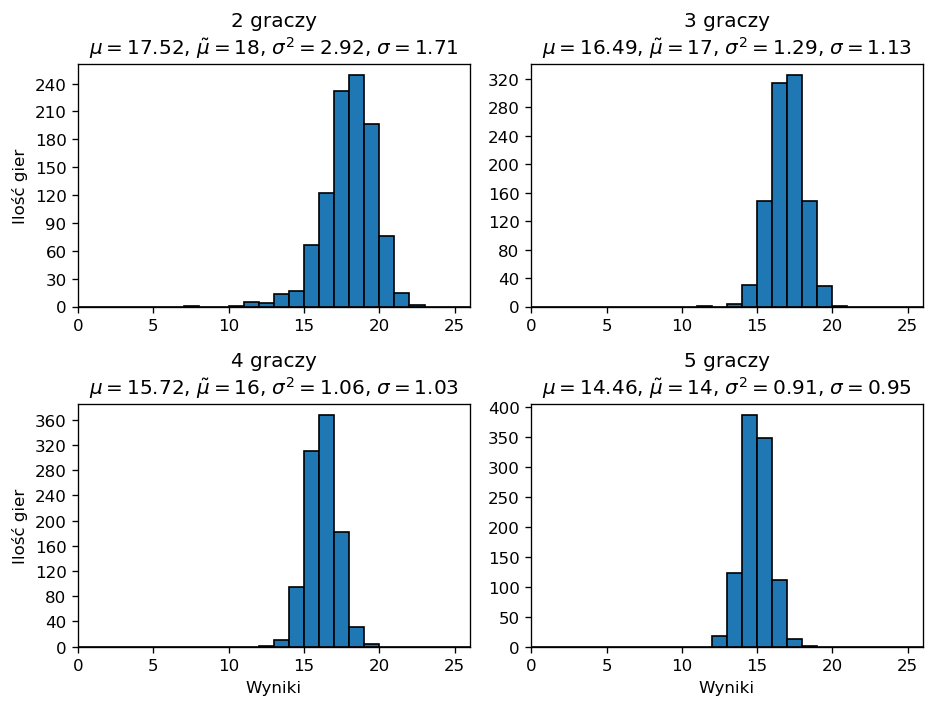
\includegraphics[width=\textwidth,height=\textheight,keepaspectratio]{Distrustful.png}
	\caption[Caption]{Wyniki agenta Distrustful (rozmiar próby: 1000 gier)}
	\label{fig:Distrustful}
\end{figure}

Mimo znacznego wzmocnienia strategii agenta SimpleDistrustful, osiągane wyniki nadal nie~zachwycają. Gracze udzielają heurystycznie wartościowych podpowiedzi, chronią krytyczne karty poprzez system wieku i~oszczędzają żetony na~wyjątkowe sytuacje -~trudno jednak doszukiwać~się między nimi głębszej współpracy, która jest kluczowa dla wysokich osiągów. Zagrywane są~wyłącznie karty inferowalnie bezpieczne, co, nawet przy bardzo ostrożnej i~wydajnej komunikacji, nie~wystarcza do~podjęcia równej walki z~szybko kurczącą~się ilością żetonów podpowiedzi. Aby przekroczyć wyczekiwany próg średniej ilości 20~punktów, potrzeba strategii, która dopuszcza pewne ryzyko.

\section{Trustful}

Poprzedników agenta Trustful nękają dwa zasadnicze problemy. Są~to: trudność związana z~efektywnym przekazywaniem informacji, a~także wystrzeganie~się zagrań, które nie są~bezpieczne. Obie te~przeszkody można pokonać poprzez ustanowienie protokołu komunikacji, który nadaje niektórym akcjom dodatkowego, implicytnego znaczenia, rozumianego przez pozostałych uczestników rozgrywki. Podpowiedzi udzielane przez agenta przekazują nie~tylko informacje o~kartach, ale i~plan działania na~kolejne tury. Aby częściowo rozwiązać problem ograniczonej ilości żetonów podpowiedzi, program potrafi, przy spełnieniu odpowiednich warunków, wykonywać ruchy, które nie~są~inferowalne, lecz mają bardzo wysokie prawdopodobieństwo bycia bezpiecznymi.

\subsection*{Nowe pojęcia}

\begin{itemize}
	\item \textbf{Obietnica}:
	
	Jeżeli agent udzieli informacji, która, zgodnie z~protokołem komunikacji, wyznacza plan zagrywania kolejnych kart, taką podpowiedź nazywamy obietnicą.
	
	\item \textbf{Komunikat}:
	
	Podpowiedź, która nie~jest obietnicą.
	
	\item \textbf{Podpowiedź ratunkowa}:
	
	Heurystycznie wartościowa podpowiedź, będąca obietnicą lub komunikatem, która jest rozważana wyłącznie dla najbliższego gracza.
	
	\item \textbf{Weto}:
	
	Akt unieważnienia efektu obietnicy karty. Jeżeli istnieje podpowiedź ratunkowa, która umożliwia danemu graczowi wykonanie jakiegoś ruchu, weto polega na~jej udzieleniu, w~przeciwnym wypadku weta dokonuje~się poprzez ujawnienie danej karty.

\end{itemize}

\subsection*{Schemat działania}

Agent posiada dwie kategorie podpowiedzi: obietnice oraz komunikaty. Ustalenie ich typu odbywa~się według następującego schematu:

\begin{enumerate}
	\item Jeżeli gracz otrzyma od~swojego bezpośredniego poprzednika podpowiedź ratunkową obejmującą kartę, która miała zostać właśnie odrzucona, podpowiedź jest komunikatem.
	\item Jeżeli gracz otrzyma od~swojego bezpośredniego poprzednika dowolną podpowiedź, gdy jedna z~kart objętych obietnicą miała zostać właśnie zagrana, ta~karta jest wetowana, a~typ podpowiedzi jest rozpatrywany ponownie, z~pominięciem tego punktu schematu.
	\item Jeżeli gracz otrzyma podpowiedź wskazującą na~numer, którego poprawne zagranie byłoby inferowalnie niemożliwe w~turze podpowiadającego gracza, podpowiedź jest komunikatem.
	\item Podpowiedź jest obietnicą.
\end{enumerate}

Agent jest złożony z~dziesięciu modułów, które są~rozważane po~kolei w~jednej z~czterech konfiguracji. Każdy moduł, poza ostatnim w~sekwencji, może zawieść. Ich kolejność zależy od~ilości posiadanych żetonów podpowiedzi:

\begin{itemize}
	\item Mniej niż 3~żetony: sekwencja 1, 2, 3, 9, 4, 5, 10 (moduły 6, 7, 8 nie są używane).
	\item Od~3~do~5 żetonów: sekwencja 1, 2, 3, 4, 5, 9, 10 (moduły 6, 7, 8 nie są używane).
	\item 6~lub~7 żetonów: sekwencja 1, 2, 3, 4, 5, 9, 6, 7, 10 (moduł 8 nie jest używany).
	\item Dokładnie 8~żetonów: sekwencja 1, 2, 3, 4, 5, 6, 7, 8, 9, 10.
\end{itemize}
Używane moduły to:

\begin{enumerate}
	\item \underline{``Necessary tip''}:

	Rozważ możliwe ruchy najbliższego gracza:
	\begin{enumerate}
		\item Jeżeli może on~niepoprawnie zagrać kartę objętą obietnicą, lecz aktualnie posiadasz inferowalnie bezpieczne zagranie, które sprawia, że~będzie ona zagrana poprawnie, wykonaj je -~w~przeciwnym wypadku zawetuj kartę.
		\item Jeżeli może on~odrzucić kartę krytyczną, lecz istnieje podpowiedź ratunkowa, która umożliwiłaby mu~wykonanie innego ruchu, udziel jej -~w~przeciwnym wypadku ujawnij kartę, priorytetyzując informację o~numerze.
	\end{enumerate}

	\item \underline{``Obvious play''}:
	
	Jeżeli posiadasz inferowalnie bezpieczne zagranie, wykonaj~je, nadając priorytet kartom o~niższych numerach.
	
	\item \underline{``Hinted play''}:

	Jeżeli posiadasz karty objęte obietnicą, których zagranie nie~może być w~oczywisty sposób niepoprawne, zagraj tę~najbardziej wysuniętą na~lewo, nadając priorytet kartom o~ujawnionym numerze i~wybierając spośród nich te, których numer jest najniższy.

	\item \underline{``Play tip''}:
	
	Jeżeli istnieje heurystycznie wartościowa podpowiedź, która umożliwi innemu graczowi inferowalnie bezpieczne zagranie (lub zagranie bazujące na~obietnicy), udziel jej.

	\item \underline{``Discard tip''}:
	
	Jeżeli istnieje heurystycznie wartościowa podpowiedź, która umożliwi innemu graczowi odrzucenie inferowalnie bezużytecznej karty, udziel jej.

	\item \underline{``Risky tip''}:
	
	Spróbuj wykonać akcję modułu numer~4 (``Play tip'') z~obniżoną karą za~błędne obietnice i~zwiększonym pułapem jakościowym.
	
	\item \underline{``Save tip''}:
	
	Jeżeli istnieje heurystycznie wartościowa podpowiedź ujawniająca kartę krytyczną, którą można wykonać w~trybie komunikatu, udziel jej, nadając priorytet graczom, którzy nie~mają inferowalnie bezpiecznego zagrania lub dobrej obietnicy, a~także preferując karty o~niższych numerach.
	
	\item \underline{``Information tip''}:
	
	Wykonaj akcję modułu numer~4 (``Play tip'') ze~zwiększoną nagrodą za~udzielanie podpowiedzi w~trybie komunikatu.
	
	\item \underline{``Obvious discard''}:
	
	Jeżeli posiadasz inferowalnie bezużyteczną kartę, odrzuć ją.

	\item \underline{``Guess discard''}:
	\begin{enumerate}
		\item Jeżeli posiadasz nieujawnione karty, odrzuć najstarszą z~nich.
		\item Jeżeli posiadasz karty, które nie~są~inferowalnie krytyczne, odrzuć najstarszą z~nich.
		\item Odrzuć najstarszą kartę.
	\end{enumerate}

\end{enumerate}

Wagi funkcji heurystycznych ponownie zostały dobrane eksperymentalnie, lecz sposób oceny akcji znacznie różni~się od~tego znanego z~agenta Distrustful. Z~racji na~ambiwalencję udzielanych typów podpowiedzi, należy uważać nie~tylko na~jakość przekazywanych informacji, ale i~ich znaczenie w~kontekście protokołu komunikacji.

Poza czynnikami wyszczególnionymi podczas analizy agenta Distrustful, na~werdykt algorytmu wpływają między innymi:

\begin{itemize}
	\item czy podpowiedź jest obietnicą,
	\item czy komunikat zostanie uznany za~obietnicę, mimo że~tego nie~chcemy,
	\item czy karta może stać~się grywalna w~turze danego gracza,
	\item czy karta jest pod działaniem efektu obietnicy,
	\item czy podpowiedź zniweczy przydatną obietnicę,
	\item czy podpowiedź jest ryzykowna,
	\item kolejność ujawnianych kart w~ręce,
	\item ilość pozostałych żetonów życia.
\end{itemize}

Podpowiadanie kart w~trybie obietnicy rzadko przebiega w~bezproblemowy sposób: karty tworzące dobry porządek w~ręce gracza to~nieczęste zjawisko. Z~tego powodu funkcje heurystyczne agresywnie zaniżają noty obietnic, których pierwszy element jest niepoprawny, lecz relaksują kary dla podpowiedzi umożliwiających co~najmniej jedno bezpieczne zagranie.

Udzielanie podpowiedzi podlega pewnemu rygorowi, lecz czasami potencjalny zysk z~udzielenia informacji o~wielu kartach naraz przeważa nad ryzykiem związanym z~niepoprawnością obietnicy. Ponieważ agent stara~się zachowywać co~najmniej jeden żeton podpowiedzi na~takie przypadki, ryzyko niefortunnego zagrania drastycznie spada. Niestety, nadal może dojść do~sytuacji, w~których gracze tracą żetony życia poprzez niepoprawne zagrania. Aby temu zapobiec, agent ogranicza zaufanie do~innych graczy, gdy w~grze pozostał ostatni żeton życia -~zagrywane są~wyłącznie te~karty objęte obietnicą, które zostały podpowiedziane pojedynczo. W~ten sposób całkowicie eliminowane jest ryzyko niebezpiecznych zagrań, lecz agent nadal nie~degeneruje swojej strategii do~tej znanej z~agenta Distrustful.

Strategia agenta nie~jest~przystosowana do~rozgrywek dwuosobowych, gdyż udzielenie dowolnej podpowiedzi wetuje kartę, która miała szansę być właśnie zagrana -~prowadzi to~do konieczności omijania systemu wetowania obietnic. Można to~osiągnąć wyłącznie poprzez wykonanie jednej z~pozostałych akcji, co~jest trudnym zadaniem, gdyż wiąże~się ono~z koniecznością dobrej znajomości własnych kart.

\subsection*{Osiągi}

\begin{figure}[H]
	\centering
	\captionsetup{format=hang}
	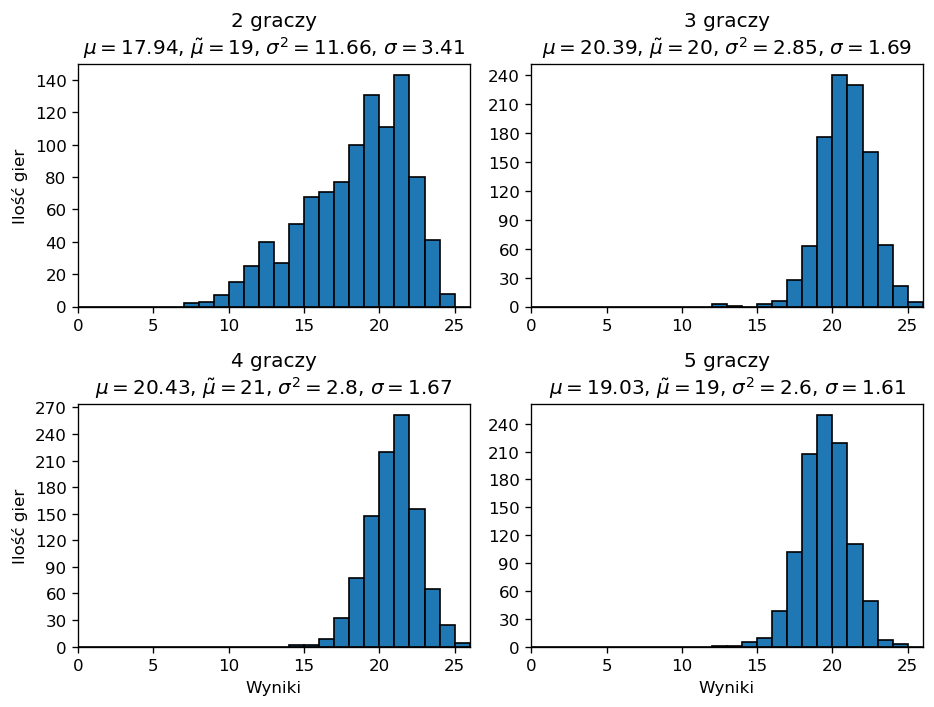
\includegraphics[width=\textwidth,height=\textheight,keepaspectratio]{Trustful.png}
	\caption[Caption]{Wyniki agenta Trustful (rozmiar próby: 1000 gier)}
	\label{fig:Trustful}
\end{figure}

Agent Trustful nie tylko potrafi przekroczyć próg 20~punktów, ale i~zdarza mu~się~wygrać: zastosowanie protokołu implicytnej komunikacji pozwoliło wynieść osiągi sztucznej inteligencji na~nowy poziom. Niestety, strategia programu nie~jest przystosowana do~rozgrywek dwuosobowych, co~objawia~się wysoką niestabilnością algorytmu. Wartym zaobserwowania faktem, który można odczytać z~wykresu, jest, występujący od~pewnego momentu rozgrywki, wykładniczy wzrost trudności uzyskiwania kolejnych punktów.

\section{BayesianTrustful}

Agent BayesianTrustful stanowi próbę odnalezienia nowych wag funkcji heurystycznych agenta Trustful, które pierwotnie zostały dobrane manualnie. W~tym celu użyliśmy bayesowskiej metody optymalizacji hiperparametrów, korzystającej z~procesów gaussowskich.

\subsection*{Podstawy teoretyczne}

Bayesowska metoda optymalizacji to~proces iteracyjny, oparty o~twierdzenie Bayesa, który korzysta z~wnioskowania statystycznego do~analizy prawdopodobieństwa hipotez. Rozważmy przestrzeń hipotez $\mathbb{H}$, której elementom $h$ przyporządkowane są~początkowe prawdopodobieństwa $P(h)$, zwane $\textit{a priori}$. Prawdopodobieństwo hipotezy $h\in\mathbb{H}$ po~dokonaniu nowej obserwacji $O$ można wyrazić wzorem $P(h|O)$, nazywanym $\textit{a posteriori}$. Metoda bayesowska pozwala na~aktualizację prawdopodobieństwa $\textit{a priori}$ hipotez w~oparciu o~nowe obserwacje. To~działanie przekłada~się~na~możliwość dokonywania wnioskowania statystycznego na~temat rozkładu funkcji, która nie~posiada wzoru jawnego.

Proces gaussowski to proces stochastyczny, który pozwala na~określenie łącznego rozkładu prawdopodobieństwa (oraz jego niepewności) wybranej rodziny nieparametrycznych funkcji $\mathbb{F}$. Polega on~na~konstrukcji prawdopodobieństw $\textit{a priori}$, które można aktualizować poprzez kolejne obserwacje, co~tworzy system przekonań o~kształcie badanych funkcji.

\begin{figure}[H]
	\centering
	\captionsetup{format=hang}
	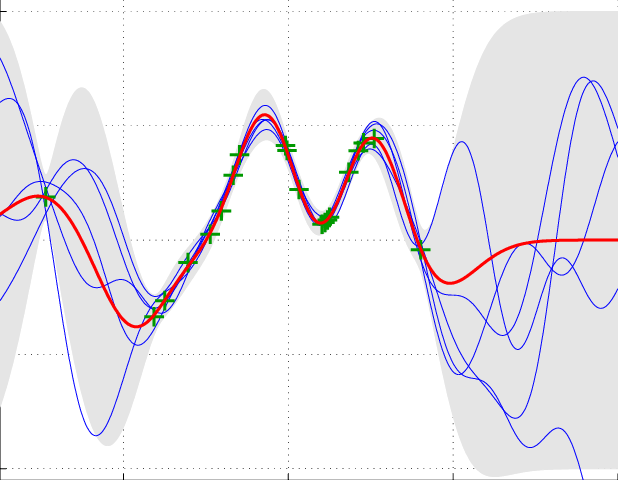
\includegraphics[width=\textwidth,height=\textheight,keepaspectratio]{Gauss.png}
	\caption[Caption]{Wizualizacja procesu gaussowskiego. Zielonymi plusami zaznaczono obserwacje, niebieskie krzywe to~poprzednie przekonania $\textit{a posteriori}$, zaś czerwona krzywa to~ich średnia wartość. Zacieniona część wykresu wyznacza niepewność modelu. Żródło: $\cite{Gauss}$}
	\label{fig:Gauss}
\end{figure}

Bayesowska metoda optymalizacji oparta o~procesy gaussowskie polega na~stworzeniu rozkładu $\textit{a priori}$ funkcji, której maksimum szukamy, a~następnie próbkowaniu jej. Nowe obserwacje pozwalają na~aktualizację prawdopodobieństw $\textit{a posteriori}$. Wraz ze~wzrostem ilości obserwacji przekonania algorytmu ulegają zmianie, a~ponieważ proces gaussowski pozwala na~identyfikację tych części funkcji, które najbardziej wymagają większej ilości obserwacji, metoda ta~minimalizuje ilość próbkowań, potrzebnych do~dalszych rozważań.

Maksymalizowana była funkcja o~27 parametrach, odpowiadających wagom używanym w~funkcjach heurystycznych. Jej wartość w~punkcie została zdefiniowana jako średnia arytmetyczna wyników uzyskanych na~przestrzeni 20~niezależnych rozgrywek. Proces optymalizacji zajął około 50~godzin.

\subsection*{Osiągi}

Aby porównać efekty optymalizacji, stworzyliśmy agentów BayesianTrustful2 oraz BayesianTrustful4, którzy przeprowadzali odpowiednio rozgrywki dwuosobowe i~czteroosobowe.

\begin{figure}[H]
	\centering
	\captionsetup{format=hang}
	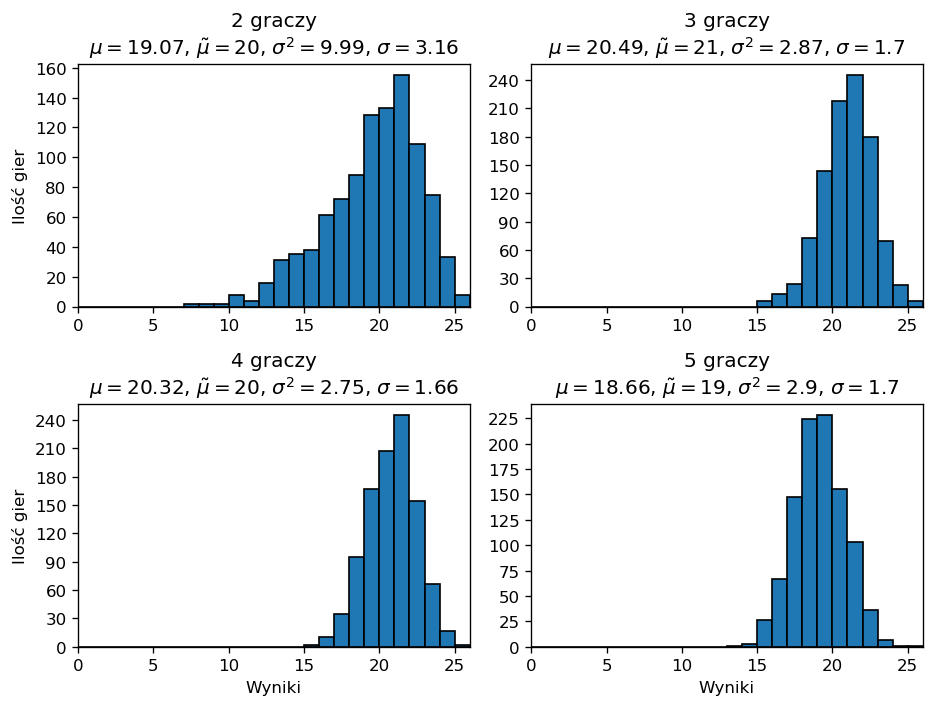
\includegraphics[width=\textwidth,height=\textheight,keepaspectratio]{BayesianTrustful2.png}
	\caption[Caption]{Wyniki agenta BayesianTrustful2 (rozmiar próby: 1000 gier)}
	\label{fig:BayesianTrustful2}
\end{figure}

Przeprowadzone testy wskazują na wzrost średniej ilości punktów dla każdego typu rozgrywki, kosztem nieznacznie zwiększonej wariancji rozgrywek trzyosobowych i~czteroosobowych. W~rozgrywkach dwuosobowych agent pokonuje wszystkich dotychczas przedstawionych agentów, którzy nie~oszukują.

Na~podstawie analizy wartości nowych wag można dociec, w~jaki sposób zmieniła~się strategia agenta BayesianTrustful2:

\begin{itemize}
	\item Moduł ``Discard tip'', pomagający graczom w~odrzucaniu bezużytecznych kart, udziela podpowiedzi wyłącznie w~sytuacji, w~której jest w~stanie częściowo ujawnić jednocześnie co~najmniej 3~karty (poprzednia wartość:~2).
	\item Moduł ``Play tip'', zarządzający podpowiedziami dotyczącymi zagrań, w~znacznie większym stopniu nagradza zagrania lawinowe, a~także jest bardziej skłonny do~udzielania mało wartościowych informacji, jeżeli częściowo ujawniają one karty o~niższych numerach. Dodatkowo, agenci nigdy nie~udzielają informacji, jeżeli wetowałyby one~poprawne zagrania.
	\item Moduły ``Risky tip'' (udzielający podpowiedzi będących nieprawidłowymi obietnicami) oraz ``Information tip'' (zarządzający komunikatami), otrzymały karę o~wysokości, która całkowicie wyklucza możliwość ich wykorzystania.
\end{itemize}

\begin{figure}[H]
	\centering
	\captionsetup{format=hang}
	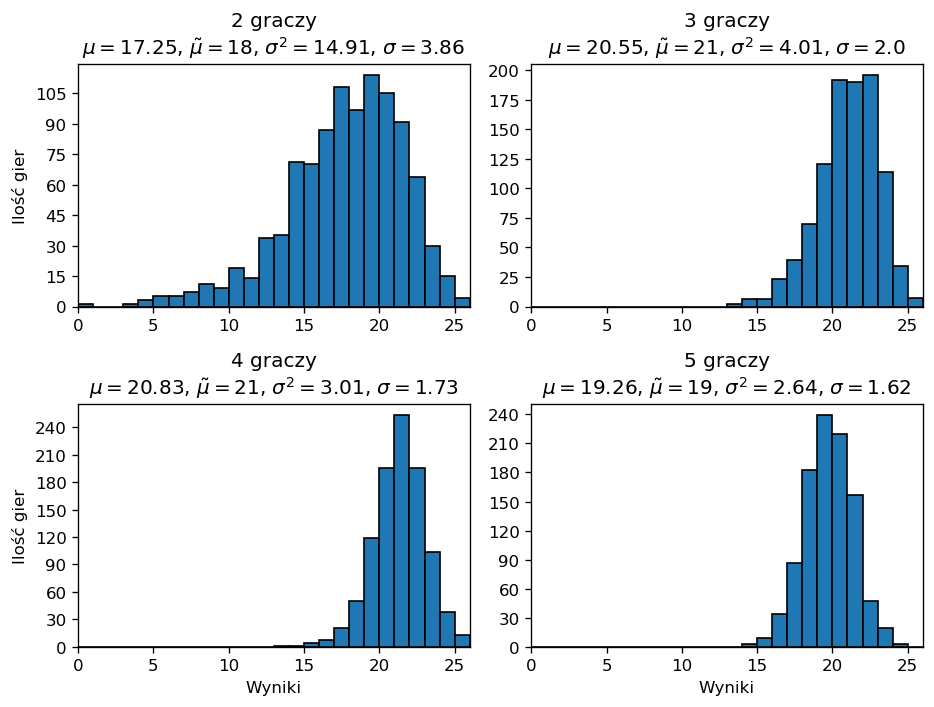
\includegraphics[width=\textwidth,height=\textheight,keepaspectratio]{BayesianTrustful4.png}
	\caption[Caption]{Wyniki agenta BayesianTrustful4 (rozmiar próby: 1000 gier)}
	\label{fig:BayesianTrustful4}
\end{figure}

Przeprowadzone testy wskazują na~niewielki wzrost średniej ilości punktów dla grup trzech, czterech i~pięciu graczy, kosztem zwiększonej wariancji. Lepsze dostosowanie wag, które pomagają przy bardziej licznych grupach, pogrąża strategię dla dwóch graczy.

Na~podstawie analizy wartości nowych wag można dociec, w~jaki sposób zmieniła~się strategia agenta BayesianTrustful4:

\begin{itemize}
	\item Moduł ``Discard tip'', pomagający graczom w~odrzucaniu bezużytecznych kart, udziela podpowiedzi wyłącznie w~sytuacji, w~której jest w~stanie częściowo ujawnić jednocześnie co~najmniej 4~karty (poprzednia wartość:~2).
	\item Moduł ``Play tip'', zarządzający podpowiedziami dotyczącymi zagrań, w~znacznie większym stopniu nagradza zagrania lawinowe, udzialanie informacji dalszym graczom oraz podpowiedzi dotyczące kart o~niższych numerach, jednocześnie drastycznie zwiększając kary za~nieprawidłowe obietnice i~marginalizując znaczenie podpowiedzi będących komunikatami.
	\item Moduł ``Risky tip'', pozwalający na~udzielanie podpowiedzi będących nieprawidłowymi obietnicami, otrzymał karę o~wysokości, która całkowicie wyklucza możliwość jego wykorzystania.
	\item Moduł ``Information tip'', pozwalający na~udzielanie podpowiedzi będących komunikatami, ma~zwiększony pułap jakościowy, co~sprawia, że~jest on~znacznie rzadziej wykorzystywany.
\end{itemize}

Podsumowując: obaj agenci są~mniej skłonni do~udzielania podpowiedzi będących komunikatami i~agresywnie penalizują nieprawidłowe obietnice. Choć prowadzi to do~uzyskania wyższej średniej punktowej, takie postępowanie może destabilizować algorytm i~powodować wzrost wariancji obserwowanych wyników, tak jak w~przypadku BayesianTrustful4.

\section{Reinforced}

Poprzednicy agenta Reinforced korzystali ze~ściśle określonych systemów regułowych. W~przeciwieństwie do~nich, agent Reinforced samodzielnie dopracowuje obieraną strategię poprzez sukcesywne rozgrywanie kolejnych partii i~wyciąganie wniosków na~temat wykonanych ruchów.

Na~początku procesu uczenia, każdej z~możliwych akcji agenta przydzielony jest taki sam priorytet, gdyż program nie~wie, który z~ruchów może być przydatny w~danym momencie rozgrywki. Wiedza o~tym, jakie zachowania są~najbardziej pożądane, jest nabywana poprzez egzekwowanie systemu kar i~nagród, nadawanych w~trakcie gry, a~także po~jej zakończeniu. Na~ich podstawie wyciągane są~wnioski, które pozwalają na~dokonywanie lepszych decyzji w~przyszłości -~zarówno w~skali makro (wybieranie jednej z~trzech akcji: zagrania, odrzucenia i~podpowiedzi), jak i~mikro (określanie szczegółów ruchu).

\subsection*{Schemat działania}

Agent posiada cztery funkcje oceniające, które pozwalają na~rozstrzyganie, które akcje powinny otrzymać najwyższe priorytety.

\begin{enumerate}
	\item Rozstrzygnij, która z~posiadanych kart powinna zostać zagrana.
	\item Rozstrzygnij, która z~posiadanych kart powinna zostać odrzucona.
	\item Rozstrzygnij, która z~możliwych do~udzielenia podpowiedzi jest najbardziej przydatna, pomijając te~z~nich, które nie ujawniają żadnych informacji.
	\item Sprawdź, które akcje zostały ocenione najlepiej, a~następnie rozstrzygnij, która z~nich powinna zostać wykonana.
\end{enumerate}

Funkcje oceniające nie~są~narzucone odgórnie. Każda z~nich wydaje werdykt w~zależności od~obecnego stanu gry, a~także wartości, które zostały wyuczone na~podstawie poprzednich decyzji, podjętych w~zbliżonych warunkach. Mechanizm ten przypomina działanie algorytmu Q-learning.

\subsection*{Model uczący}

Najwyższe osiągi i~największą swobodę nauki można osiągnąć poprzez przekazywanie funkcjom oceniającym struktur, które dokładnie odwzorowują obserwowany stan rozgrywki. Dane, które musiałyby być zawarte w~takim obiekcie, to~między innymi: kolejność kart w~rękach graczy, status stosów zagranych kart, listy odrzuconych oraz niedobranych kart, a~także historia ruchów poszczególnych graczy. Niestety, ze~względu na~bardzo dużą ilość unikalnych stanów gry, użycie takiego obiektu jest niepraktyczne, gdyż długość procesu uczenia stałaby~się nieakceptowalna. Należałoby rozważyć ponad $10^{12}$ stanów -~zakładając, że~potrafimy zbadać w~ciągu jednej sekundy około 500 z~nich, pojedyncze odwiedzenie każdego elementu drzewa stanów trwałoby ponad 63~lata. Aby zredukować złożoność algorytmu, zdecydowaliśmy~się na~upraszczanie stanów gry przy użyciu funkcji heurystycznych. Pod uwagę brane są~wyłącznie informacje niezbędne do~efektywnego rozpoznawania ogólnych sytuacji, w~których może znaleźć~się agent.

Informacje o~stanie gry są~przechowywane jako kolekcja wektorów, które zawierają zestaw danych o~wybranym obiekcie gry. Informacje są~przechowywane w~formie liczbowej z~ograniczonego zakresu, co~pozwala na~zredukowanie liczby stanów rozgrywki. Wyróżniamy trzy rodzaje kontenerów o~(między innymi) następujących składowych:

\begin{enumerate}
	\item Pojedyncze karty aktualnego gracza (około $10^5$ unikalnych stanów):
		\begin{itemize}
			\item stopień ujawnienia karty,
			\item czy istnieje ryzyko, że~karta jest krytyczna,
			\item czy karta jest najstarsza,
			\item ilość kart, które zostały ujawnione w~tym samym momencie, co~rozpatrywana kartą,
			\item ilość stosów, których najwyższy numer jest niższy od~numeru rozpatrywanej karty,
			\item ilość pozostałych żetonów podpowiedzi.
		\end{itemize}
	\item Możliwe do~udzielenia podpowiedzi (około $4*10^5$ unikalnych stanów):
		\begin{itemize}
			\item ilość ujawnianych kart, które można bezpiecznie zagrać,
			\item ilość ujawnianych kart, które będzie można w~przyszłości bezpiecznie zagrać,
			\item ilość ujawnianych kart, które można inferowalnie bezpiecznie odrzucić,
			\item ilość ujawnianych kart, które zostaną w~pełni ujawnione,
			\item czy podpowiedź obejmuje kartę, która może rozpocząć zagranie lawinowe,
			\item czy podpowiedź obejmuje najstarszą kartę w~ręce gracza,
			\item czy podpowiedź obejmuje jakąkolwiek kartę krytyczną,
			\item odległość gracza udzielającego podpowiedzi od~gracza, któremu podpowiedź jest udzielana.
		\end{itemize}
	\item Możliwe do~wykonania akcje (około $10^5$ unikalnych stanów):
		\begin{itemize}
			\item ilość pozostałych żetonów podpowiedzi,
			\item ilość pozostałych żetonów życia,
			\item czy talia jest pusta,
			\item oceny najlepszych akcji z~poszczególnych kategorii.
		\end{itemize}
\end{enumerate}

Składowe pierwszych dwóch kontenerów są~od siebie całkowicie niezależne. Ponieważ wartości ostatniego kontenera zależą od~werdyktu funkcji oceniających ruchy, dwa identyczne stany rozgrywki mogą zostać ocenione na~różne sposoby. Powoduje to, że~kontener akcji dostarcza agentowi najmniej pewnych informacji.

Funkcja oceniająca to~mapowanie, które przyjmuje odpowiednie kontenery, a~następnie zwraca numeryczną ocenę rozpatrywanego ruchu. Agent dysponuje czterema funkcjami oceniającymi: po~jednej na~każdą z~akcji (zagraj kartę, odrzuć kartę, udziel podpowiedzi innemu uczestnikowi rozgrywki), a~także ostatnią, która dokonuje ostatecznej decyzji o~ruchu.

Początkowo, wartości liczbowe zwracane przez funkcje oceniające zawierają się w~przedziale $[0,1]$. Aby zachować balans pomiędzy potrzebą eksploracji nowych stanów i~wysokimi osiągami, ostatecznie wyrażane są~one za~pomocą wzoru ${S+c\sqrt{\frac{\ln (N+1)}{p}}}$, gdzie $S$~to~początkowa wartość funkcji oceniającej, $c$~to~parametr eksploracji (ustalony na~$\sqrt{2}$), $N$~to ilość odwiedzin aktualnego stanu gry, z~kolei $p$~to~ilość kar, który otrzymał rozważany stan gry. Wzór ten~jest odmianą formuły UCT (``Upper Confidence Bound~1 applied to~trees''), używanej m.in. w~algorytmie Monte Carlo Tree Search\cite{UCT}.

Po~dokonaniu analizy heurystycznej ruchów, wykonywana jest akcja, która otrzymała najwyższą notę. Aby wymusić dodatkowe losowe błądzenia, agent ma~stałą szansę na~wykonanie arbitralnego ruchu, która wynosi 1\%. Funkcjonalność ta~jest aktywna wyłącznie wtedy, gdy program znajduje~się w~trybie nauki.

Na~koniec każdej z~tur, agent rozważa efekty wybranej akcji. Jeżeli program wykonał poprawne zagranie lub odrzucił bezużyteczną kartę, funkcje oceniające ten ruch są~nagradzane. Bonus otrzymują także funkcje, które zdecydowały o~udzieleniu podpowiedzi dotyczącej danej karty. Podobnie, jeżeli zagranie było niepoprawne lub została odrzucona karta krytyczna (bądź taka, którą można było zagrać), funkcje są~karane. Z~uwagi na~trudność natychmiastowego oszacowania poprawności akcji udzielenia podpowiedzi, te~ruchy są~oceniane dopiero po~zakończeniu rozgrywki.

W~zależności od~tego, czy po~ukończeniu partii agent uzyskał wynik wyższy od~mediany punktów z~ostatniego tysiąca rozgrywek, wszystkie akcje dokonane w~trakcie gry są~nagradzane lub karane. Zmiana jest wprost proporcjonalna do~różnicy pomiędzy uzyskanym wynikiem a~medianą. Funkcja oceniająca, która dokonuje wyboru głównej akcji, korzysta z~tego mechanizmu w~największym stopniu.

Ponieważ funkcje oceniające są~ze~sobą silnie skorelowane, ocena stanu rozgrywki może diametralnie~się zmieniać w~zależności od~aktualnie przyjętej strategii. Z~tego powodu program pamięta dla każdego ze~stanów jedynie 400 ostatnich kar i~nagród, a~funkcje nadają wyższe wagi tym z~nich, które są~najnowsze.

Opisany model uczący był tworzony empirycznie, za~pomocą metody prób i~błędów, a~jego forma w~znacznej mierze wynika z~naszego zrozumienia gry Hanabi.

\subsection*{Osiągi}

Aby unaocznić efektywność opisanych metod uczących, stworzyliśmy dwa skrajnie różne środowiska, w~których agent wypracowywał swoje strategie. Agenci nazwani Reinforced2 rozgrywali partie dwuosobowe, zaś agenci Reinforced4 -~czteroosobowe. W~obu przypadkach kolejne partie były rozgrywane do~momentu, gdy osiągi agentów przestały wykazywać~się szczególnymi zmianami. Cały proces, w~trakcie którego agenci sumarycznie rozegrali blisko pół miliona gier, zajął około dwunastu godzin.

Podjęliśmy nieudaną próbę utworzenia trzeciego środowiska, w~którym pojedynczy agent Reinforced uczył~się gry z~czterema agentami Trustful. Ostatecznie nie~doszło do~jego realizacji, gdyż włączenie do~rozgrywki stosunkowo powolnych agentów Trustful spowalniało proces nauki prawie dziesięciokrotnie.

Strategia wypracowana przez agentów jest wyjątkowo trudna do~zrozumienia, gdyż proces uczenia doprowadził do~powstania ezoterycznego protokołu komunikacji. Manualna analiza kilku rozgrywek pozwoliła jednak na~wyszczególnienie kilku powtarzających~się zachowań:
\begin{itemize}
	\item Agenci preferują udzielanie obiektywnie wartościowych podpowiedzi ponad zagrywanie własnych kart, nawet, jeśli są~one bezpieczne, o~ile są~w~posiadaniu wystarczająco wysokiej ilości żetonów podpowiedzi. Jest to~szczególnie widoczne w~zachowaniu agenta Reinforced2.
	\item Udzielenie informacji o~pojedynczej karcie jest najczęściej odbierane przez pozostałych agentów jako sygnał do~jej zagrania.
	\item Agenci często udzielają podpowiedzi, które ujawniają wiele kart jednocześnie. Pozostali uczestnicy rozgrywki nie~uznają takiej podpowiedzi za~jakikolwiek sygnał, w~zamian oczekując na~nowe informacje. Ponownie, jest to~technika wykorzystywana głównie przez agenta Reinforced2.
	\item Gdy agent nie~posiada w~ręce kart, które można inferowalnie bezpiecznie odrzucić, najczęściej odrzuca nie~najstarszą, a~najmłodszą kartę.
\end{itemize}

\begin{figure}[H]
	\centering
	\captionsetup{format=hang}
	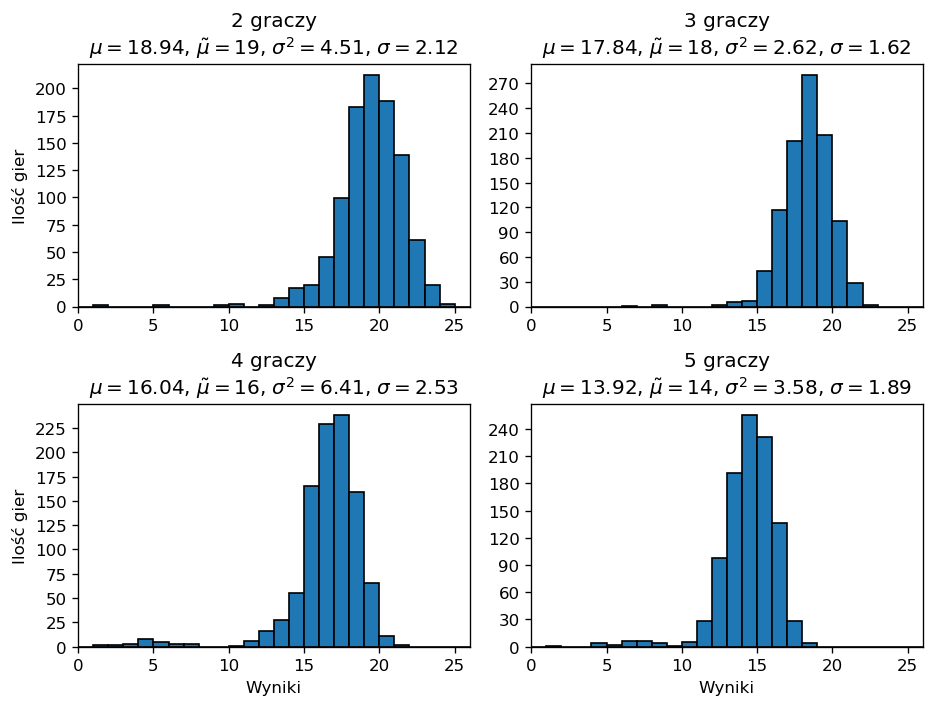
\includegraphics[width=\textwidth,height=\textheight,keepaspectratio]{Reinforced2.png}
	\caption[Caption]{Wyniki agenta Reinforced2 (rozmiar próby: 1000 gier)}
	\label{fig:Reinforced2}
\end{figure}

Agent Reinforced2, który trenował granie partii dwuosobowych, osiąga w~nich wyniki niewiele niższe od~BayesianTrustful2. Jednocześnie, mimo chaotycznego procesu formułowania strategii, zachowuje on~zaskakująco wysoką stabilność. Niestety, jak można było przewidywać, wraz~ze wzrostem liczby graczy agent uzyskuje coraz niższe wyniki. Ponadto, nigdy nie~udaje mu~się zdobyć maksymalnej ilości 25~punktów.

\bigskip

\begin{figure}[H]
	\centering
	\captionsetup{format=hang}
	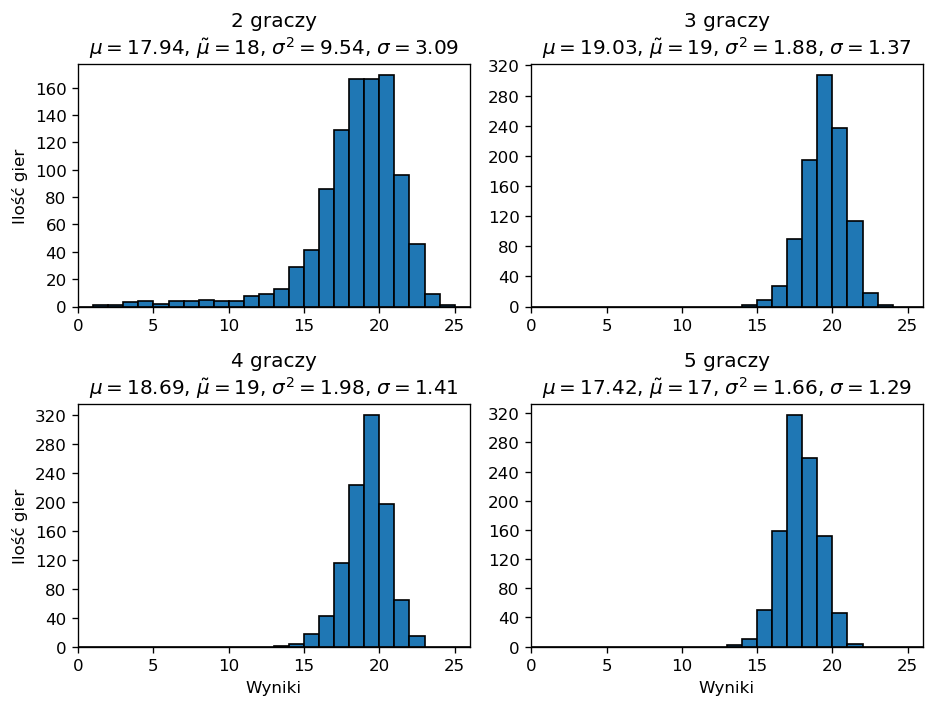
\includegraphics[width=\textwidth,height=\textheight,keepaspectratio]{Reinforced4.png}
	\caption[Caption]{Wyniki agenta Reinforced4 (rozmiar próby: 1000 gier)}
	\label{fig:Reinforced4}
\end{figure}

W~przypadku agenta Reinforced4, wypracowana strategia jest znacznie mniej podatna na~zmiany w~liczbie graczy. Choć agent nie~osiąga w~partiach dwuosobowych wyników, które pozwoliłyby mu~konkurować z~bliźniaczym algorytmem czy agentem BayesianTrustful2, pokonuje w~nich wszystkich innych agentów, którzy nie~oszukują. W~pozostałych testach sytuuje~się on~pomiędzy agentami Distrustful a~Trustful, jednocześnie wyróżniając~się bardzo wysoką stabilnością wdrażanych strategii.

\chapter{Podsumowanie wyników agentów}
 
\begin{table}[H]
	\centering
	\captionsetup{format=hang}
	\begin{tabular}{ r|c|c|c|c| }		
 		\multicolumn{1}{r}{}		
 		 & \multicolumn{1}{c}{2 graczy}		
 		 & \multicolumn{1}{c}{3 graczy}		
 		 & \multicolumn{1}{c}{4 graczy}		
 		 & \multicolumn{1}{c}{5 graczy} \\		
 		\cline{2-5}		
 		Cheater & 20.5 (2.59) & 22.27 (2.04) & 21.73 (2.07) & 21.94 (2.0) \\		
 		\cline{2-5}		
 		SmartCheater & 24.72 (0.79) & 24.91 (0.41) & 24.89 (0.41) & 24.85 (0.44) \\		
 		\cline{2-5}		
 		Erratic & 1.45 (1.5) & 1.32 (1.39) & 1.3 (1.36) & 1.34 (1.34) \\
 		\cline{2-5}		
 		StoppedClock & 5.74 (2.62) & 6.25 (2.2) & 5.31 (1.91) & 4.51 (1.69) \\
 		\cline{2-5}		
 		SimpleDistrustful & 13.37 (3.0) & 15.48 (1.3) & 15.06 (1.09) & 14.02 (1.0) \\
 		\cline{2-5}		
 		Distrustful & 17.52 (1.71) & 16.49 (1.13) & 15.72 (1.03) & 14.46 (0.95) \\
 		\cline{2-5}		
 		Trustful & 17.94 (3.41) & 20.39 (1.69) & 20.43 (1.67) & 19.03 (1.61) \\
 		\cline{2-5}		
 		BayesianTrustful2 & $\textbf{19.07 (3.16)}$ & 20.49 (1.7) & 20.32 (1.66) & 18.66 (1.7) \\
 		\cline{2-5}		
 		BayesianTrustful4 & 17.25 (3.86) & $\textbf{20.55 (2.0)}$ & $\textbf{20.83 (1.73)}$ & $\textbf{19.26 (1.62)}$ \\
 		\cline{2-5}		
 		Reinforced2 & 18.94 (2.12) & 17.84 (1.62) & 16.04 (2.53) & 13.92 (1.89) \\
 		\cline{2-5}		
 		Reinforced4 & 17.94 (3.09) & 19.03 (1.37) & 18.69 (1.41) & 17.42 (1.29) \\
 		\cline{2-5}		
 	\end{tabular}		
 	\caption{Średnia wyników agentów sztucznej inteligencji (rozmiar każdej z~prób: 1000 gier). W~nawiasach podano odchylenie standardowe. Najlepsze wyniki zostały pogrubione.}		
 	\label{table:summary}		
 \end{table}
 
 Agent BayesianTrustful4 uzyskał aż~trzy z~czterech najwyższych średnich punktów spośród agentów, którzy nie~oszukują. Lepszym wyborem do~partii na trzech graczy byłby jednak agent BayesianTrustful2 -~choć jego wynik jest nieco niższy, różnica w~odchyleniu standardowym jest na~tyle znacząca, by~móc chcieć go~wybrać w~celu uzyskania bardziej stabilnego przebiegu rozgrywki. Podobne rozumowanie skłania do~zastąpienia BayesianTrustful2 agentem Reinforced2 w~rozgrywkach dwuosobowych.

\chapter{Niestandardowe modele rozgrywki}

\section{Dwa oblicza drużyn Hanabi}

Prezentowanie możliwości dotychczas przedstawionych agentów polegało na~pomyśle umieszczania ich w~homogenicznych środowiskach, na~które składało~się wiele kopii jednego agenta. Gwarantowało to, że~wszyscy uczestnicy rozgrywki posiadali jednolitą strategię. W~naturalny sposób nasuwa~się pytanie: co~może~się wydarzyć, kiedy do~partii zasiądą gracze o~różnych schematach działania?

Rozgrywki mieszane, znane także jako potyczki XY, stanowią ciekawy problem w~kontekście sztucznej inteligencji grającej w~Hanabi, gdyż wymagają pogodzenia dwóch antytetycznych konceptów: konieczności współpracy oraz braku wspólnego planu działania. Niepewność poczynań innych graczy zmienia problematykę całej gry: implicytna komunikacja staje~się niemożliwa, a~gracze w~każdej chwili mogą wykonać akcje, które nie mają sensu z~punktu widzenia współuczestników rozgrywki, co~skutecznie paraliżuje większość strategii. Dobrym sposobem na~uzyskanie wysokich wyników nie~jest już kooperacja, a~maksymalne ograniczenie zaufania do~innych graczy. W~przypadku agentów sztucznej inteligencji, którzy nie~potrafią dostosowywać~się do~zmieniających warunków tak, jak robią to~ludzie, zredefiniowanie formuły rozgrywki może prowadzić do~zaskakujących rezultatów.

\section{Potyczki XY}

Przeprowadziliśmy testy rozgrywek, w~których gracze występowali w~różnych konfiguracjach. Ponieważ istnieją dziesiątki możliwych ustawień, wybraliśmy z~nich te, które uznaliśmy za~najciekawsze. Partie na~pięciu graczy niewiele różnią~się od~tych na~czterech graczy, toteż zostały one pominięte.

\subsection*{Partie na dwóch graczy}

\begin{figure}[H]
	\centering
	\captionsetup{format=hang}
	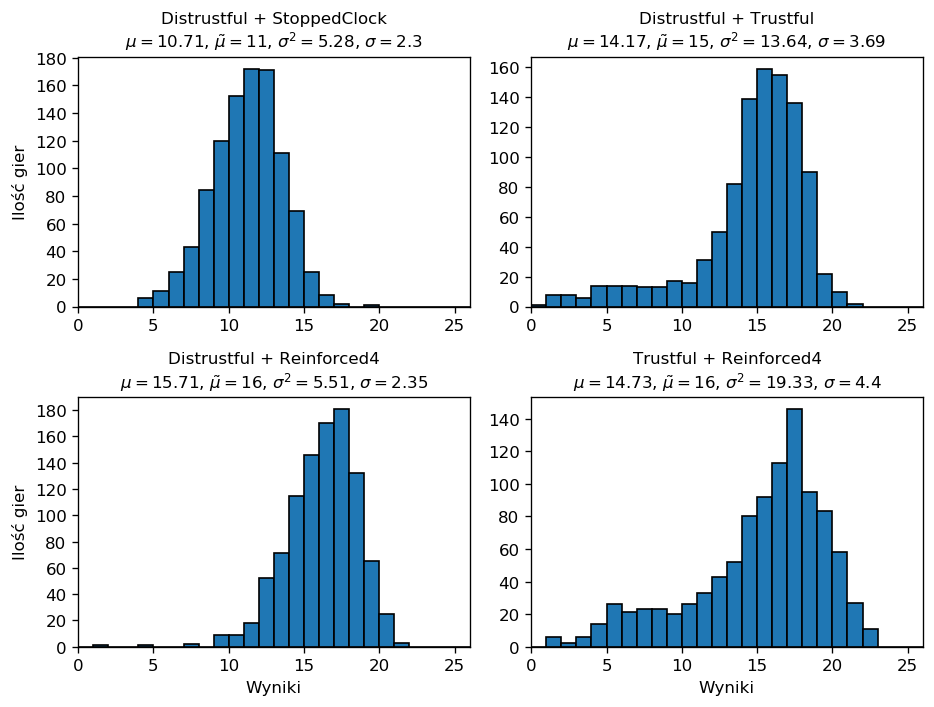
\includegraphics[width=\textwidth,height=\textheight,keepaspectratio]{XY2.png}
	\caption[Caption]{Wyniki potyczek XY dla dwóch graczy (rozmiar próby: 1000 gier)}
	\label{fig:XY2}
\end{figure}

Agenci Distrustful oraz StoppedClock używają strategii, które dobrze ze~sobą współgrają. Zagrywane są~wyłącznie karty bezpieczne, a~pomiędzy graczami nie~istnieje żaden protokół komunikacji, który mógłby zostać przypadkowo złamany. Ich połączenie skutkuje dosyć stabilnymi wynikami, mimo przypadkowości akcji dokonywanych przez agenta StoppedClock.

Jak można było przewidywać, protokół komunikacji agenta Trustful źle współgra z~graczami, którzy go~nie stosują: agent Distrustful udziela podpowiedzi, które są~nadinterpretowywane przez Trustful, co~prowadzi do~niepoprawnych zagrań. Problem potęguje~się, gdy drugim uczestnikiem rozgrywki jest agent Reinforced4 -~posługuje~się on~nietypową strategią, co~czasami prowadzi do~zaskakująco wysokich wyników, lecz w~większości przypadków kończy~się dezorientacją agenta Trustful i~szybką przegraną.

Połączenie agentów Distrustful oraz Reinforced4 daje ciekawy rezultat: mimo różnych strategii, średnia osiąganych wyników oscyluje blisko osiągów agenta Distrustful. Zachowanie Reinforced4, z~powodu braku innych graczy, którzy rozumieliby implicytne informacje, zdegenerowało~się do~poziomu bliskiego agentowi Distrustful.

\subsection*{Partie na trzech graczy}

\begin{figure}[H]
	\centering
	\captionsetup{format=hang}
	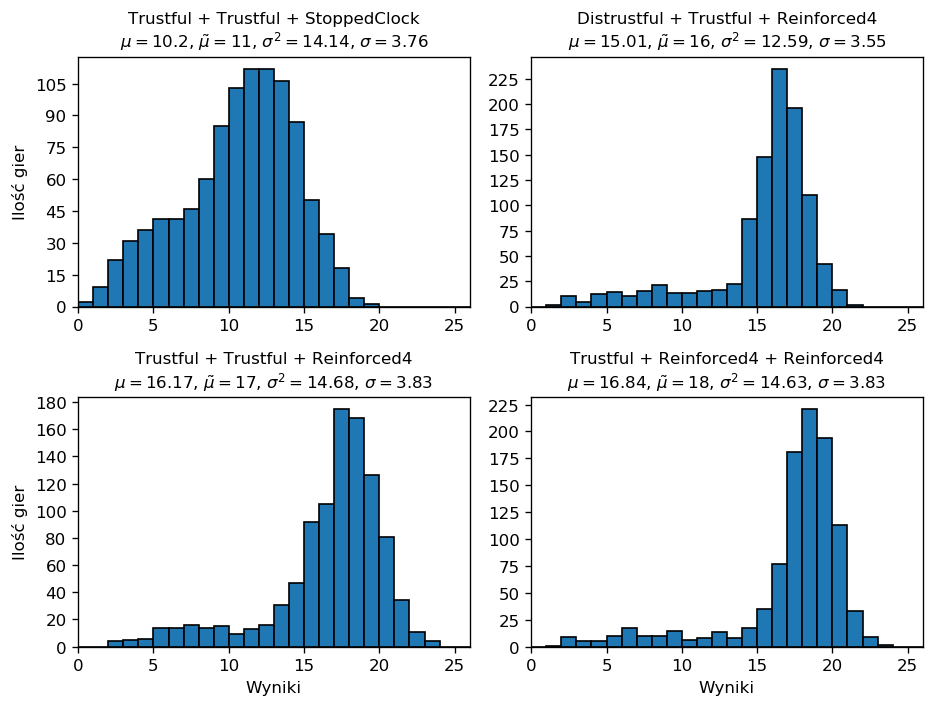
\includegraphics[width=\textwidth,height=\textheight,keepaspectratio]{XY3.png}
	\caption[Caption]{Wyniki potyczek XY dla trzech graczy (rozmiar próby: 1000 gier)}
	\label{fig:XY3}
\end{figure}

Nawet, gdy w~grze z~agentami Trustful znajduje~się tylko jeden gracz, który łamie zasady protokołu komunikacji, losowe podpowiedzi prowadzą do~porażającej ilości szybkich porażek. Po~raz kolejny potwierdza~się fakt, że~agent Trustful nie~sprawdza~się w~potyczkach~XY: jego kooperacyjna strategia prowadzi do~powstawania błędnych przekonań, których inni agenci nie~są~w~stanie na~czas skorygować, by~zapobiec nieszczęściu.

Podobna, chociaż mniej ekstremalna sytuacja ma~miejsce, gdy dwóch agentów Trustful próbuje współpracować z~agentem Reinforced4. Rozumie on~część protokołu komunikacji, gdyż stosuje technikę podpowiadania pojedynczych kart, lecz nie~ma~pojęcia o~systemie obietnic. Często doprowadza to~do~wetowania kolejnych kart i~zmusza drugiego agenta Trustful do~udzielania dodatkowych informacji. Rozgrywki, w~których uczestniczy dwóch agentów Reinforced4 oraz jeden agent Trustful to~przypadek symetryczny, gdyż tym razem to~Trustful rozumie tylko część protokołu komunikacji.

Wymieszanie trzech różnych agentów okazuje~się nie~być tragiczne w~skutkach: w~porównaniu do~rozgrywki na~dwóch graczy, w~której uczestniczyli wyłącznie Trustful oraz Reinforced4, dodatkowy gracz w~postaci agenta Distrustful pełni rolę arbitra, który balansuje niedobory w~przekazywanych informacjach.

\subsection*{Partie na czterech graczy}

\begin{figure}[H]
	\centering
	\captionsetup{format=hang}
	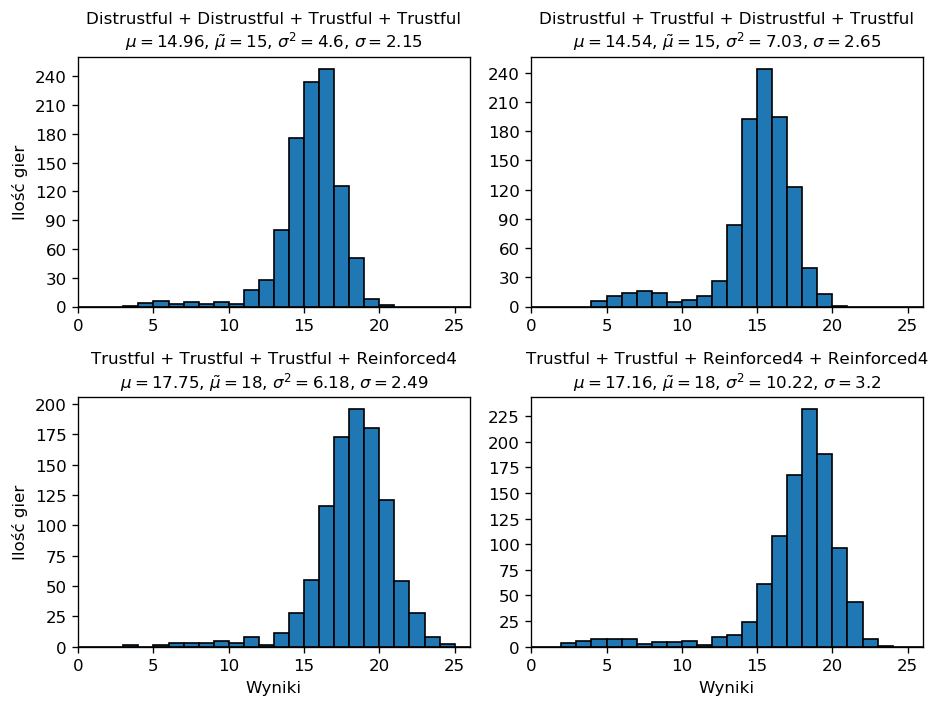
\includegraphics[width=\textwidth,height=\textheight,keepaspectratio]{XY4.png}
	\caption[Caption]{Wyniki potyczek XY dla czterech graczy (rozmiar próby: 1000 gier)}
	\label{fig:XY4}
\end{figure}

Okazuje~się, że~nie~tylko dobór agentów, ale i~ich kolejność może mieć znaczenie dla przebiegu gry. Ustawienie agentów Trustful obok siebie skutkuje możliwością korekty obietnic, które zostały nieświadomie wystosowane przez pozostałych agentów uczestniczących w~rozgrywce. Ułożenie agentów naprzemiennie nie~pozwala na~zastosowanie tej części protokołu komunikacji, co~objawia się~niższymi wynikami, a~także większą niestabilnością uzyskiwanych wyników.

Wraz ze~wzrostem liczby graczy, różnice pomiędzy protokołami komunikacji są~bardziej oczywiste -~nawet, gdy mają one pewne cechy wspólne. Zastąpienie jednego z~agentów Trustful przez~Reinforced4 powoduje znaczne zwiększenie wariancji ilości uzyskiwanych punktów. Fenomen ten nie~występował w~partiach na~trzech graczy, gdzie wymiana Trustful-Reinforced4 skutkowała mało istotnymi zmianami.

\section{Podsumowanie}

Agenci, którzy wykorzystują wysublimowane strategie, są~w~znacznie większym stopniu podatni na~niekorzystne sytuacje, wynikające ze~specyfiki mieszanych rozgrywek. W~potyczkach~XY największą stabilność uzyskują strategie bazujące na~wnioskowaniu, które nie~polegają na~sygnałach od~innych graczy. Potwierdzają to~zarówno wyniki eksperymentów, jak i~badania nad drużynami ad-hoc w~Hanabi, przeprowadzone w~pracy pt. \textit{``Diverse Agents for Ad-Hoc Cooperation in Hanabi''}\cite{AdHoc}.

\bigskip

\begin{figure}[H]
	\centering
	\captionsetup{format=hang}
	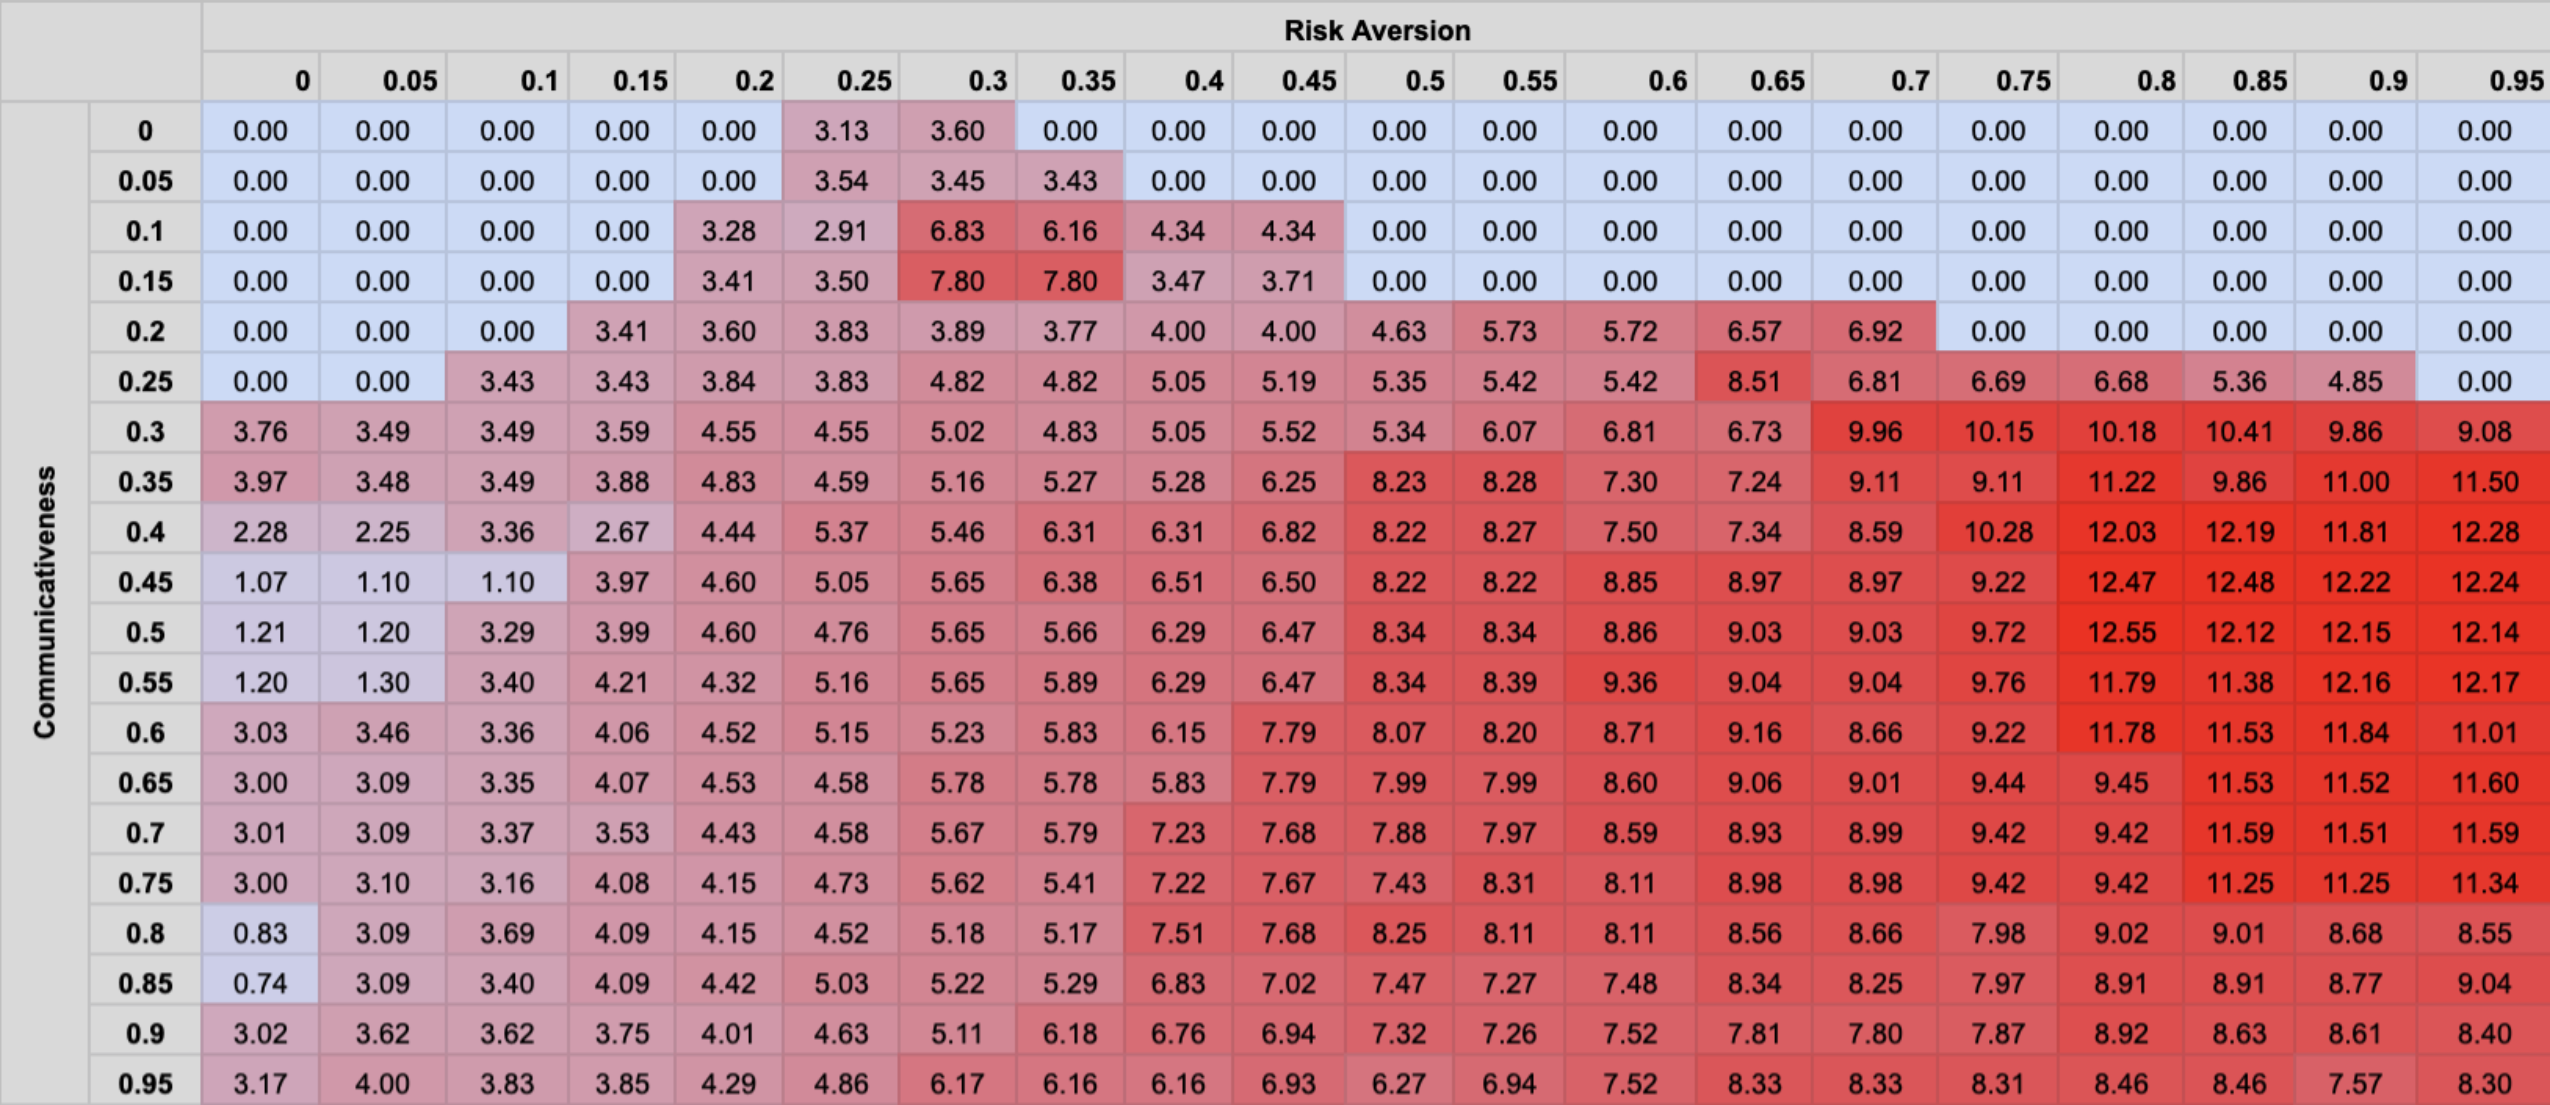
\includegraphics[width=\textwidth,height=\textheight,keepaspectratio]{ad-hoc.png}
	\caption[Caption]{Średnie wyniki agentów o~zadanych parametrach Communicativeness (komunikatywność) oraz Risk Aversion (unikanie ryzyka). Badanie było przeprowadzone poprzez uśrednienie wyników serii rozgrywek dwusobowych (rozmiar każdej z~prób: 1000 gier), w~których drugi z~graczy był wybierany z~puli 326 agentów o~pozostałych kombinacjach parametrów. Źródło: \cite{AdHoc}}
	\label{fig:ad-hoc}
\end{figure}

W~drużynach ad-hoc premiowana jest wyważona strategia. Agenci osiągają znacznie lepsze wyniki, gdy unikają ryzyka, lecz nie~mogą czynić tego kosztem ograniczania komunikacji -~Hanabi, z~racji bycia grą kooperacyjną, wymaga pewnej formy współpracy. Rozgrywki mieszane zmuszają nie~do~maksymalizacji wyników, a~minimalizacji możliwych do~poniesienia strat. Aby nie~pozwolić współuczestnikom rozgrywki na~popełnianie tragicznych w~skutkach błędów, należy ich kierować ku~dobrym zagraniom, jednocześnie na~pierwszym miejscu stawiając swoje poczynania. Najlepszym sposobem na~uzyskiwanie wysokich wyników jest ograniczona współpraca, która zakłada, że~inni gracze mogą wykonywać akcje sprzeczne z~przyjętą logiką.

\chapter{Wnioski}

Problem gry w~Hanabi to~złożone zagadnienie, które nie~bez powodu rozbudza ciekawość zarówno pasjonatów gier planszowych, jak i~matematyków czy informatyków. Jego trudność można określić mianem interdyscyplinarnej: w~zależności od~sposobu postawienia problemu, techniki jego analizy oraz rozwiązania diametralnie~się różnią. Stworzenie agentów sztucznej inteligencji, którzy potrafiliby grać w~Hanabi na~poziomie mistrzowskim, jest wyjątkowo skomplikowanym zadaniem, wymagającym zastosowania niestandardowych rozwiązań.

Zaprezentowani agenci sztucznej inteligencji nie~osiągnęli wyników, które mogłyby konkurować z~programami wykorzystującymi złożone obliczeniowo techniki. Stanowią oni jednak dowód możliwości tworzenia szybkich i~skutecznych rozwiązań zawiłych problemów algorytmicznych, korzystających nie~z~kolosalnej mocy współczesnych komputerów, lecz~dobrej znajomości zadania, z~którym dane jest~się nam mierzyć.

Tworzenie agentów sztuczej inteligencji grających w~Hanabi to~zagadnienie, które unaocznia potęgę ludzkiej intuicji. Algorytmy regułowe, choć w~znacznej mierze zdeprecjonowane i~zastąpione przez nowe techniki tworzenia sztucznej inteligencji, przypominają, że~pewne problemy można rozwiązywać nie~tylko z~pomocą wyspecjalizowanych narzędzi, ale i~nietuzinkowych pomysłów.

\chapter{Dalsze badania}

Choć agenci Reinforced2 oraz Reinforced4 osiągają zadowalające wyniki, mogą one zostać usprawnione poprzez rozszerzenie lub modyfikację uproszczonych stanów gry. Trudność tego zadania jest bezpośrednio powiązana z~problemem wykładniczego przyrostu długości procesu nauki, który postępuje wraz z~dodawaniem kolejnych składowych obiektów stanów.

W~pracy nie~zbadano możliwości stworzenia agenta, który dostosowywałby swój sposób postępowania w~zależności od~akcji, których dokonywaliby inni uczestnicy rozgrywki. Algorytm, który potrafiłby dynamicznie dostosowywać swoją strategię, mógłby osiągać bardzo wysokie wyniki zarówno w~potyczkach XY, jak i~grach, w~których uczestniczy człowiek.

Protokół komunikacji agenta Trustful został oparty o~nasze własne spostrzeżenia, zdobyte podczas obserwacji rozgrywek ludzkich graczy. Nie wykluczamy istnienia bardziej zaawansowanych strategii (przykładowo: opartych o~obserwacje zachowań profesjonalnych graczy Hanabi), które pozwoliłyby na~uzyskanie wyższych wyników.

\appendix
\chapter{Korzystanie z projektu}

\section{Instalacja zależności}
Aby skorzystać ze~wszystkich możliwości programu, potrzebne będzie zainstalowanie środowiska uruchomieniowego Python~3. Projekt był testowany przy użyciu wersji 3.7.4 na~następujących systemach operacyjnych:
\begin{itemize}
	\item Windows 10, kompilacja 17763
	\item MacOS~Catalina 10.15.2
	\item Ubuntu 18.04.3 LTS
\end{itemize}

\subsection{Windows}

Należy otworzyć powłokę CMD lub PowerShell, przejść do~głównego katalogu projektu, a~następnie wykonać następującą komendę:
\begin{verbatim}
    $ python3 -m pip install -r requirements-windows.txt
\end{verbatim}

\subsection{MacOS}

Należy otworzyć jedną z~powłok systemu Unix (przykładowo: bash, zsh), przejść do~głównego katalogu projektu, a~następnie wykonać następującą komendę:
\begin{verbatim}
    $ python3 -m pip install -r requirements-macos.txt
\end{verbatim}

\subsection{Ubuntu Linux}

Należy otworzyć jedną z~powłok systemu Unix (przykładowo: bash, zsh), a~następnie wykonać następujące komendy:
\begin{spverbatim}
    $ sudo add-apt-repository ppa:kivy-team/kivy
    $ sudo apt update
    $ sudo apt install python3-pip python3-tk python3-kivy python3-sdl2
    $ python3 -m pip install bayesian-optimization
\end{spverbatim}

\subsection{Inne systemy operacyjne}

Należy zainstalować biblioteki \emph{bayesian-optimization} oraz \emph{Kivy}$\footnote{Instrukcja instalacji biblioteki Kivy: \href{https://kivy.org/doc/stable/gettingstarted/installation.html}{\textbf{link}} (term. wiz. 03.02.2020)}$. Instalacji pierwszej z~nich można dokonać poprzez wykonanie w~powłoce systemowej następującej komendy:
\begin{verbatim}
    $ python3 -m pip install bayesian-optimization
\end{verbatim}

\section{Uruchamianie projektu}

Aby uruchomić graficzny interfejs użytkownika, należy otworzyć powłokę systemu operacyjnego, przejść do~głównego katalogu projektu, a~następnie wykonać następującą komendę:
\begin{verbatim}
    $ python3 hanabi.py
\end{verbatim}

\noindent Spowoduje to~pojawienie się~menu wyboru agentów, które pozwala na~rozpoczęcie nowej rozgrywki w~Hanabi.

\section{Dodatkowe funkcje}

Główny katalog projektu zawiera programy, które pozwalają na~kontynuowanie jego rozwoju, a~także powtórzenie przeprowadzonych eksperymentów:
\begin{itemize}
	\item Aby rozpocząć proces uczenia własnego agenta Reinforced, wystarczy uruchomić plik o~nazwie $learning\_example.py$.
	\item Program odpowiedzialny za~optymalizację hiperparametrów metodą bayesowską zawarty jest w~pliku $bayesian\_optimization.py$.
	\item Wyniki eksperymentów dokonywanych na~agentach można znaleźć w~notatniku $benchmark.ipynb$. Do otworzenia pliku potrzebne będzie zainstalowanie programu Jupyter Notebook$\footnote{Instrukcja instalacji programu Jupyter Notebook: \href{https://jupyter.org/install}{\textbf{link}} (term. wiz. 03.02.2020)}$.
\end{itemize}

\begin{thebibliography}{4}

\bibitem{DeepBlue} M. Campbell, A. J. Hoane Jr., F. Hsu, \textit{Deep Blue}, 2002. URL: 
\href{https://core.ac.uk/download/pdf/82416379.pdf}{\textbf{link}} (term. wiz. 03.02.2020)

\bibitem{NP-Complete} J.-F Baffier i in., \textit{Hanabi is NP-complete, Even for Cheaters who Look at Their Cards}, 2017. URL: 
\href{https://arxiv.org/pdf/1603.01911.pdf}{\textbf{link}} (term. wiz. 03.02.2020)

\bibitem{MCTS} A. Lerer, H. Hu, J. Foerster, N. Brown, \textit{Building AI that can master complex cooperative games with hidden information}, 2019. URL: 
\href{https://ai.facebook.com/blog/building-ai-that-can-master-complex-cooperative-games-with-hidden-information/}{\textbf{link}} (term. wiz. 03.02.2020)

\bibitem{Mario} T. Murphy, \textit{The First Level of Super Mario Bros. is Easy with Lexicographic Orderings and Time Travel $\ldots$after that it gets a little tricky.}, 2013. URL: 
\href{http://www.cs.cmu.edu/~tom7/mario/mario.pdf}{\textbf{link}} (term. wiz. 03.02.2020)

\bibitem{HatPlayer} B. Bouzy, \textit{Playing Hanabi Near-Optimally}, 2017. URL: 
\href{http://helios.mi.parisdescartes.fr/~bouzy/publications/bouzy-hanabi-2017.pdf}{\textbf{link}} (term. wiz. 03.02.2020)

\bibitem{Gauss} Fernando Pérez-Cruz i in., \textit{Gaussian Processes for Nonlinear Signal Processing: An Overview of Recent Advances}, 2013. URL: 
\href{https://www.researchgate.net/publication/260637079_Gaussian_Processes_for_Nonlinear_Signal_Processing_An_Overview_of_Recent_Advances}{\textbf{link}} (term. wiz. 03.02.2020)

\bibitem{UCT} L. Kocsis, C. Szepesvári, \textit{Bandit Based Monte-Carlo Planning}, 2006. URL: 
\href{https://link.springer.com/content/pdf/10.1007/11871842_29.pdf}{\textbf{link}} (term. wiz. 03.02.2020)

\bibitem{AdHoc} R. Canaan i in., \textit{Diverse Agents for Ad-Hoc Cooperation in Hanabi}, 2019. URL: 
\href{https://arxiv.org/pdf/1907.03840.pdf}{\textbf{link}} (term. wiz. 03.02.2020)

\bibitem{OurInspiration} N. Bard i in., \textit{The Hanabi Challenge: A New Frontier for AI Research}, 2019. URL: 
\href{https://arxiv.org/pdf/1902.00506.pdf}{\textbf{link}} (term. wiz. 03.02.2020)

\end{thebibliography}

\end{document}
